\chapter{Σχεδιασμός και υλοποίηση}
\label{chap:implementation}

Όπως είδαμε στο προηγούμενο κεφάλαιο κανένα unikernel \EN{framework} δεν υποστηρίζει
την κλήση συστήματος fork και επομένως εφαρμογές που χρησιμοποιούν τη
συγκεκριμένη κλήση δεν μπορούν να υποστηριχτούν από αυτά. Στο πλαίσιο, λοιπόν,
της παρούσας διπλωματικής εργασίας δημιουργήσαμε ένα μηχανισμό που
υλοποιεί τις κλήσεις συστήματος fork και pipe σε KVM hypervisor. Ο στόχος ήταν
να διατηρηθεί το single process χαρακτηριστικό των unikernels. Για το λόγο
αυτό το αποτέλεσμα της κλησης fork, δεν είναι η δημιουργία μία νέας διεργασίας
στο υπάρχον unikernel, αλλά η εκκίνηση ενός unikernel, ίδιου με το αρχικό. 

Επιπλέον, υλοποιήθηκε και ένας inter-vm communication μηχανισμός, στα πρότυπα
της κλήσης συστήματος pipe. Δηλαδή δύο εικονικά μηχανήματα μπορούν να
επικοινωνούν μεταξύ τους, όπως δύο διεργασίες επικοινωνούν μεταξύ τους, μέσω της
κλήσης συστήματος pipe, σε ένα λειτουργικό σύστημα γενικού σκοπού. 

Στο παρών κεφάλαιο περιγράφουμε αναλυτικά τους δύο αυτούς μηχανισμούς. Το
κεφάλαιο χωρίζεται σε δύο μέρη, ένα για το μηχανισμό pipe και ένα για το
μηχανισμό fork. Σε κάθε μέρος περιγράφεται αναλυτικά τόσο ο μηχανισμός, όσο και
η διαδικασία και τα στάδια μέχρι την τελική υλοποίηση τους.

\newpage
\section{Μηχανισμός pipe}

Σύμφωνα με το POSIX ο ορισμός της κλήσης συστήματος pipe έχει ως εξής:
\begin{lstlisting}[numbers=none,  xleftmargin=.2\textwidth, xrightmargin=.2\textwidth]
int pipe(int fildes[2]);
\end{lstlisting}
Ο μηχανισμός pipe που υλοποιήθηκε ακολουθεί τον ορισμό του
POSIX. Πιο συγκεκριμένα μία κλήση στη συγκεκριμένη συνάρτηση δημιουργεί ένα pipe
μεταξύ των δύο εικονικών μηχανημάτων και δημιουργεί δύο νέους file descriptors.
Οι δύο αυτοι file descriptors αποθηκεύονται στις παραμέτρους fildes[0] και
fildes[1]. Ο πρώτος file descriptor αφορά το read κομμάτι του pipe, ενώ ο
δεύτερος το write κομμάτι του pipe. Η τιμή που επιστρέφει η κλήση συστήματος
είναι 0, αν η δημιουργία του pipe ήταν επιτυχής, ενώ διαφορετικά θα επιστραφεί
-1 και η μεταβλητή errno περιέχει την τιμή του σφάλματος.

Η ανάγνωση από το pipe γίνεται χρησιμοποιώντας τον πρώτο file descriptor από τις
παραμέτρους της κλήσης. Τα δεδομένα διαβάζονται με FIFO (first in first out)
σειρά. Ενώ αν δεν υπάρχουν δεδομένα στο pipe τότε η κλήση "μπλοκάρει" μέχρι να
προκύψουν δεδομένα από το write άκρο του pipe. Η εγγραφή στο pipe γίνεται
χρησιμοποιώντας το δεύτερο file descriptor από τις παραμέτρους της κλήσης. Η
εγγραφή στο pipe μπορεί να μπλοκάρει αν δεν υπάρχει χώρος στο pipe. Επιπλέον
μπορεί να αποτύχει αν όλα τα file descriptos για ανάγνωση από το pipe έχουν
κλείσει με το σφάλμα EPIPE. 

\subsection{Στάδια υλοποίησης}

Η υλοποίηση του συγκεκριμένου μηχανσιμού έγινε σε 3 στάδια, τα οποία αναλύονται
παρακάτω. 

\subsubsection{Στάδιο 1 - επίπεδο εφαρμογής}

%%Στο πρώτο στάδιο, δημιουργήσαμε μία επικοινωνία μεταξύ των unikernels,
%%χρησιμοποιώντας TCP/IP sockets. Όπως φαίνεται στην παρακάτω εικόνα \ref{fig4_1}
%%όλη η εργασία για τη δημιουργία της επικοινωνίας γινόταν μέσα από την  εφαρμγοή
%%που εκτελούνταν στο unikernel. Δεδομένου της χρήσης των sockets, κάποιο
%%unikernel θα έπρεπε να είχε το ρόλο του server και το άλλο το ρόλο του client.
%%Όπως γίνεται εύκολα κατανοητό, ο συγκεκριμένος μηχανισμός απαιτεί την ύπαρξη
%%σύνδεσης σε κάποιο κοινό δίκτυο για τα δύο εικονικα μηχανήματα.

Στο πρώτο στάδιο, υλοποιήσαμε το pipe ως μία συνάρτηση που καλείται από την
εφαμρογή. Η συνάρτηση αυτή χρησιμοποιεί TCP/IP sockets για να εγκαθιδρύσει την
επικοινωνία μεταξύ ρων δύο εφαρμογών. Συγκεκριμένα χρησιμοποιούνται δύο sockets,
ένα για την αποστολή δεδομένων και ένα για την παραλαβή. Οι file descriptors των
των δύο αυτών sockets, είναι και οι τιμές που αποθηκεύονται στις μεταβλητές
fildes[0] και fildes[1]. Στην παρακάτω εικόνα \ref{fig4_1} φαίνεται σχηματικά η
υλοποίηση.

\begin{figure}[htp]
\centering
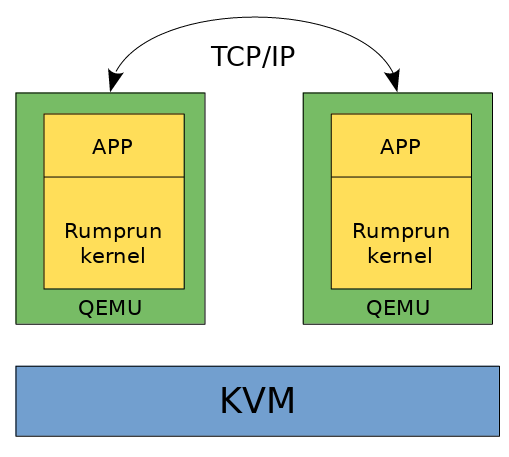
\includegraphics[scale=0.7]{figures/pipe_stage1_function.png}
\caption{Πρώτο στάδιο υλοποίησης μηχανισμού pipe\label{fig4_1}}
\end{figure}

Όπως γίνεται εύκολα κατανοητό η συγκεκριμένη υλοποίηση απαιτεί την ύπαρξη
δικτύου ανάμεσα στα δύο εικονικά μηχανήματα. Επιπλέον, λόγω της χρήσης των
sockets, δεν υλοποιήθηκε όλα τα semantics του pipe. Έτσι ακόμα και αν δεν
υπάρχει ανοιχτό read άκρο στο pipe, οποιαδήποτε εγγραφή στο pipe θα είναι
επιτυχής. Ακόμα, οποιαδήποτε εγγραφή μπορεί να μπλοκάρει μόνο αν ο παραλήπτης
δεν μπορεί να δεχτεί άλλα δεδομένα. Αντιθέτως τα semantics του άκρου ανάγνωσης
του pipe διατηρήθηκαν καθώς και στην περίπτωση των sockets, αν δεν υπάρχουν
δεδομένα προς ανάγνωση η αντίστοιχη κλήση "μπλοκάρει". 

Για να υλοποιηθεί η συνάρτηση pipe, ακολουθήθηκε η ίδια διαδικασία που
ακολουθείται από μία εφαρμογή για να επικοινωνήσει με κάποια άλλη μέσω δικτύου.
Η διαφορά είναι ότι η εφαρμογή έχει το ρόλο του server και του client
ταυτόχρονα. Για αυτό το λόγο χρησιμοποιήθηκαν δύο sockets, ένα για κάθε ρόλο. 
Στην παρακάτω εικόνα \ref{fig4_2} φαίνεται η αλληλουχία κλήσεων συστήματος για
την εγκαθίδρυση της επικοινωνίας (server/client). 

%%O συγκεκριμένος μηχανισμός επικοινωνίας είναι ακριβώς ίδιος με αυτό που
%%χρησιμοποιούν δύο εφαρμογές για να επικοινωνήσουν μεταξύ τους. Ο τρόπος με τον
%%οποίο δημιουργείται ο μηχανισμός με τις ανάλογες κλήσεις συστήματος φαίνεται
%%στην εικόνα \ref{fig4_2}. Όπως φαίνεται από τη μεριά του o client χρειάζεται να
%%ανοίξει ένα socket, να συνδεθεί με το server χρησιμοποιώντας την connect(). Από
%%τη δικιά του μεριά ο server, μετά τη δημιουργία του socket το δεσμεύει σε μία
%%συγκεκριμένη θύρα χρησιμοποιώντας την bind, θέτει το συγκεκριμένο socket ως
%%passive socket ώστε να δεχτεί νέες συνδέσεις με τη listen() και περιμένει κάποια
%%νέα σύνδεση μπλοκάροντας στην accept(). Το συγκεκριμένο στάδιο αποσκοπούσε
%%κυρίως στην περαιτέρω εξοικείωση με το rumprun unikernel framework. Στη συνέχεια
%%η ενδοεπικοινωνία γινόταν γράφοντας και διαβάζοντας στα file descriptors που
%%είχαν δημιουργηθεί από την παραπάνω διαδικασία. 

\begin{figure}[htp]
\centering
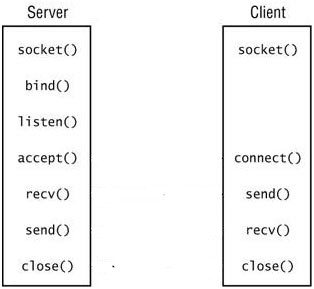
\includegraphics[scale=0.7]{figures/Server_client_syscalls_tcp_ip_socket.jpg}
\caption{Αλληλουχία κλήσεων για επικοινωνία μέσω TCP/IP sockets \label{fig4_2}}
\end{figure}

Η συνάρτηση pipe, λοιπόν ακολουθεί και τις δύο διαδικασίες που φαίνονται
(server/client). Αυτό όμως προξενεί ένα πρόβλημα κατά τη δημιουργία της
επικοινωνίας. Αν και οι δύο εφαρμογές ακολουθήσουν την παραπάνω ακολουθία
κλήσεων τότε θα δημιουργηθεί αδιέξοδο, καθώς και οι 2 θα έχουν κολλήσει στην
κλήση accept, περιμένοντας κάποια σύνδεση. Ο τρόπος με τον οποίο επιλύθηκε το
παραπάνω πρόβλημα είναι ως εξής. Μία από τις δύο εφαρμογές να εκτελεί πρώτα τις
κλήσεις που αφορούν το client κομμάτι και μετά αυτές που αφορούν το server.
Αντίθετα η άλλη εφαρμογή, πρώτα εκτελεί τις κλήσεις που αφορούν το server και
ύστερα αυτές που αφορούν το client μερος. 

\subsubsection{Στάδιο 2 - pipe ως system call με UDP sockets}

Στο δεύτερο στάδιο, υλοποιήσαμε το μηχανισμό του pipe μέσα στον πυρήνα του
rumprun. Ουσιαστικά μετατρέψαμε το function call του προηγούμενου σταδίου σε
system call. Σε αντίθεση με πριν, η επικοινωνία γίνεται μέσω UDP sockets, οπότε
και είναι απαραίτητη η ύπαρξη δικτύου. Η επιλογή του πρωτοκόλλου UDP έναντι του
TCP, έγινε για την πιο εύκολη δημιουργία και χρήση sockets στον πυρήνα του
rumprun. Ο συγκεκριμένος μηχανισμός δίνει τη δυνατότητα να υπάρχει επικοινωνία
μεταξύ δύο ξεχωριστών unikernels, ακόμα και αν αυτά δε μοιράζονται τον ίδιο
host, μέσω μίας κλήσης συστήματος παρόμοια με την pipe(). Με αυτό τον τρόπο, οι
εφαρμογές δε χρειάζονται να τροποποιηθούν σε μεγάλο βαθμό, από την αρχική τους
έκδοση. Στην παρακάτω εικόνα ~\ref{fig4_3} φαίνεται σχηματικά η υλοποίηση.

\begin{figure}[htp]
\centering
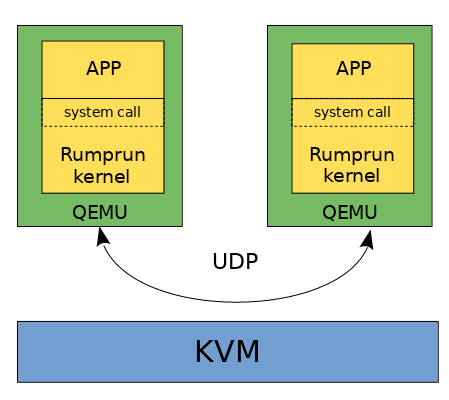
\includegraphics[scale=0.7]{figures/pipe_stage2.png}
\caption{Δεύτερο στάδιο υλοποίησης μηχανισμού pipe\label{fig4_3}}
\end{figure}

Όσον αφορά τη χρήση του μηχανισμού, αυτή γίνεται ακολουθώντας την ίδια
διαδικασία με τη χρήση της κλήσης pipe σε ένα UNIX σύστημα. Στις παραμέτρους
fildes[0], fildes[1], αποθηκεύονται οι δύο file descriptors που θα
χρησιμοποιηθούν για την ανάγνωση και εγγραφή αντίστοιχα. Σε περίπτωση επιτυχίας
επιστρέφεται η τιμή 0, ενώ σε αντίθετη περίπτωση, στη μεταβλητή errno
αποθηκεύεται ο κωδικός του σφάλματος. Δεδομένου, ότι η επικοινωνία γίνεται με
UDP sockets, τα semantics είναι ίδια με το προηγούμενο στάδιο. Μία σημαντική
διαφορά, είναι ότι πρέπει να καθοριστεί η διεύθυνση IP του unikernel με το οποίο
θα εγκαθιδρυθεί η επικοινωνία. Για το λόγο αυτό, μετά την κλήση της pipe() θα
πρέπει μέσω της ioctl στο file descriptor της εγγραφής 
\begin{lstlisting}[numbers=none,  xleftmargin=.05\textwidth, xrightmargin=.05\textwidth]
ioctl(fildes[1], SETIPADDR, htonl(IP_ADDRESS));
\end{lstlisting}
Η μορφή της IP διεύθυνσης θα πρέπει να είναι σε network byte order
και για αυτό το σκοπό μπορεί να χρησιμοποιηθεί η συνάρτηση htonl.
Ο τρόπος που λειτουργεί ο μηχανισμός έχει ως εξής:
\begin{enumerate}
	\item Αρχικά καλώντας την pipe, επιστρέφονται τα δύο απαραίτητα file
		descriptors, ένα για εγγραφή και ένα για ανάγνωση.
	\item Στη συνέχεια, πρεπει να οριστεί η διεύθυνση IP, στην οποία θέλουμε
		να στείλουμε τα δεδομένα. Αυτό γίνεται μέσω της προαναφερθείσας
		ioctl κλήσης. 
	\item Η εφαρμογή στέλνει δεδομένα χρησιμοποιώντας την κλήση write() και
		το file descriptor που αντιπροσωπεύει το άκρο εγγραφής του pipe.
	\item H εφαρμογή λαμβάνει δεδομένα χρησιμοποιώντας την κλήση read() και
		το file descriptor που αντιπροσωπεύει το άκρο ανάγνωσης του pipe.
\end{enumerate}

Η μεταφορά του μηχανισμού στον πυρήνα του rumprun απαιτούσε και τις ανάλογες
αλλαγές στις συναρτήσεις που χρησιμοποιήθηκαν, καθώς πλέον ο προγραμματισμός
γινόταν εντός του πυρήνα. Ο πυρήνας που χρησιμοποιεί το rumprun είναι αυτός του
NetBSD και σε σχέση με τον τρόπο που χρησιμοποιούνται τα sockets σε userspace,
διαφέρει με τον αντίστοιχο σε kernelspace. Ο συγκεκριμένος μηχανισμός
χρησιμοποιεί ένα struct, στο οποίο αποθηκεύονται το socket, το file descriptor
και η διεύθυνση IP του παραλήπτη. 
\begin{lstlisting}[numbers=none,  xleftmargin=.2\textwidth, xrightmargin=.2\textwidth]
struct pipe_data {
	struct socket *so;
	uint32_t ip;
	int fd;
};
\end{lstlisting}
Παρακάτω, περιγράφεται τι γίνεται μέσα στον πυρήνα όταν εκτελούνται οι παραπάνω
κλήσεις. 
\begin{enumerate}
	\item pipe: Αρχικά, δημιουργούνται δύο sockets με την socreate, ένα για
		αποστολή και ένα για παραλαβή δεδομένων και αποθηκεύονται στα
		αντίστοιχα πεδία του struct pipe\_data. Το socket που θα
		χρησιμοποιηθεί για ανάγνωση γίνεται bind στη θύρα 23456 με την
		sobind,	επιτρέποντας συνδέσεις από κάθε IP. Στη συνέχεια,
		δημιουργούνται τα 2 file descriptors που θα χρησιμοποιούνται από
		την εφαρμογή. Τα file descriptos, από τη μεριά του πυρήνα
		αντιπροσωπεύονται από τις δομές file\_t. Στις δομές
		αυτές αποθηκεύεται και το struct pipe\_data που αναφέρθηκε
		προηγουμένως. Αν όλα έχουν πάει καλά, προστίθονται τα δύο file
		descriptors στην εφαρμογή και επιστρέφει με επιτυχία η pipe.
	\item ioctl: Όταν καλείται η ioctl με το command SETIPADDR, αποθηκεύεται
		στο πεδίο ip του pipe\_data η τιμή που έχει περαστεί ως τρίτη
		παράμετρος στην ioctl.
	\item write: Αρχικά αρχικοποιείται το struct sockaddr\_in, το οποίο
		λαμβάνει την IP του παραλήπτη από το πεδίο ip του pipe\_data.
		Στη συνέχεια χρησιμοποιώντας τη sosend, στέλνονται τα δεδομένα
		μέσα από το socket.
	\item read: Με τη χρήση της soreceive, διαβάζονται τυχόν δεδομένα στο
		socket. Αν δεν υπάρχουν δεδομένα η soreceive μπλοκάρει μέχρι να
		προκύψουν.
\end{enumerate}

Στον πυρήνα του NetBSD, τυχόν δεδομένα που μεταφέρονται από userspace σε
kernelspace αποθηκεύονται στο struct uio. Τόσο η soreceive, όσο και η sosend,
δίνουν τη δυνατότητα να χρησιμοποιηθεί το συγκεκριμένο struct και συνεπώς δεν
υπάρχει ανάγκη για παραπάνω αντιγραφές των δεδομένων. Η διαδικασία για την
εισαγωγή μία νέας κλήσης συστήματος στο rumprun, είναι ακριβώς ίδια με αυτή που
θα χρησιμοποιηθεί για την εισαγωγή μία κλήσης συστήματος στον πυρήνα του NetBSD,
με ένα επιπλέον βήμα. Αφού εισαχθεί η κλήση συστήματος στο NetBSD, πρέπει να
εισαχθεί στο αρχείο src-netbsd/sys/rump/librump/rumpkern η κλήση συστήματος.
Σε αυτό το σημείο, καλό είναι να ξανααναφερθεί ότι στα unikernels δεν υπάρχει
διαχωρισμός μεταξύ userspace και kernelspace, ωστόσο οι συγκεκριμένοι όροι
χρησιμοποιούνται για να γίνει διαχωρισμός μεταξύ του κώδικα μίας οποιασδήποτε
εφαρμογής και του κώδικα του πυρήνα του unikernel.

%% -----------------------------------------------------------------------------
%% ------------------------ Deutero stadio me device ---------------------------
%% -----------------------------------------------------------------------------

%%Στο δεύτερο στάδιο, υλοποιήσαμε το μηχανισμό, μέσα στον πυρήνα του rumprun. Όπως
%%και στο προηγούμενο στάδιο, έτσι και εδώ η επικοινωνία γίνεται μέσψ TCP/IP
%%sockets, συνεπώς είναι απαραίτητη η ύπαρξη δικτύου. Βέβαια ο συγκεκριμένος
%%μηχανισμός μπορεί να χρησιμοποιηθεί για την επικοινωνία rumprun unikernels που
%%δε βρίσκονται στον ίδιο host. Ο τρόπος με τον οποίο επιλέχθηκε να γίνει αυτό
%%είναι μέσω μίας ψευδοσυσκευής. Στην παρακάτω εικόνα \ref{fig4_3} φαίνεται 
%%σχηματικά η υλοποίηση.  
%%
%%\begin{figure}[htp]
%%\centering
%%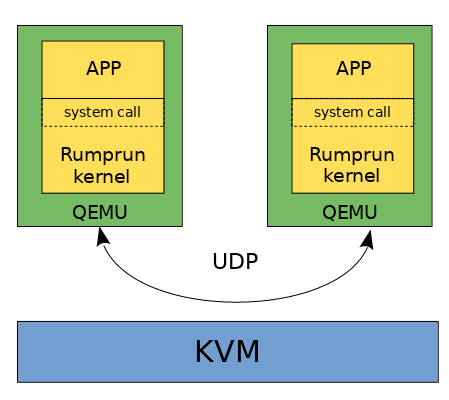
\includegraphics[scale=0.7]{figures/pipe_stage2.png}
%%\caption{Δεύτερο στάδιο υλοποίησης μηχανισμού pipe\label{fig4_3}}
%%\end{figure}
%%
%%Στο επίπεδο της εφαρμογής, ο μηχανισμός είναι διαθέσιμος μέσω της συσκευής
%%/dev/comso. Ανοίγωντας τη συγκεκριμένη συσκευή, η εφαρμογή έχει τη δυνατότητα να
%%στέλνει και να λαμβάνει δεδομένα, γράφοντας και διαβάζοντας αντίστοιχα στη
%%συγκεκριμένη συσκευή. Ουσιαστικά το pipe έχει μετατραπεί σε μία ψευδοσυσκευή που
%%μπορεί να επικοινωνήσει μέσω TCP/IP sockets, με άλλες εφαρμογές. Ο τρόπος με τον
%%οποίο υλοποιήθηκε ο μηχανισμός, αλλάζει τον ορισμό του pipe, καθώς μέσω του
%%ίδιου file descriptor, η εφαρμογή μπορεί να γράψει ή να διαβάσει δεδομένα. Τέλος
%%τα semantics είναι ίδια με το προηγούμενο στάδιο. 
%%
%%Η μεταφορά του μηχανισμού στον πυρήνα του rumprun απαιτούσε και τις ανάλογες
%%αλλαγές στις συναρτήσεις που χρησιμοποιήθηκαν, καθώς πλέον ο προγραμματισμός
%%γινόταν εντός του πυρήνα. Ο πυρήνας που χρησιμοποιεί το rumprun είναι αυτός του
%%NetBSD και σε σχέση με τον τρόπο  που χρησιμοποιούνται τα sockets σε userspace,
%%διαφέρει με τον αντίστοιχο σε kernelspace. Ο τρόπος που λειτουργεί ο μηχανισμός
%%φαίνεται στην εικόνα \ref{fig4_4} και μία σύντομη περιγραφή του έχει ως εξής:
%%\begin{enumerate}
%%	\item Αρχικά η εφαρμογή χεησιμοποιεί την open για να ανοίξει τη συσκευή.
%%		Από τη μεριά του πυρήνα, αυτό έχει ως αποτέλεσμα τη δημιουργία
%%		του socket που θα χρησιμοποιηθεί για την επικοινωνία. Η
%%		δημιουργία του socket γίνεται χρησιμοποιώντας τη sosocket().
%%	\item Η εφαρμογή στέλνει δεδομένα χρησιμοποιώντας την κλήση write() και
%%		το file descriptor που αντιπροσωπεύει την ανοιχτή συσκευή comso.
%%		Από τη μεριά του πυρήνα, όταν λαμβάνεται το συγκεκριμένο αίτημα
%%		χρησιμοπποιείται η sosend, για να σταλούν τα δεδομένα μέσω του
%%		socket στον προορισμό.
%%	\item H εφαμρογή λαμβάνει δεδομένα χρησιμοποιώντας την κλήση open() και
%%		το file descriptor που αντιπροσωπεύει την ανοιχτή συσκευή comso.
%%		Από τη μεριά του πυρήνα, όταν λαμβάνεται το συγκεκριμένο αίτημα
%%		γίνεται bind το socket, σε μία συγκεκριμένη θύρα, με τη sobind,
%%		και στη συνέχεια, χρησιμοποιείται η soreceive. Η συγκεκριμένη
%%		συνάρτηση του πυρήνα του NetBSD περιμένει να υπάρξει μία νέα
%%		σύνδεση και στη συνέχεια περιμένει να λάβει δεδομένα που έχουν
%%		σταλεί στο συγκεκριμένο socket.
%%	\item Τέλος, όταν η εφαρμογή κλείσει το αρχείο που αντιπροσωπεύει την
%%		ψευδοσυσκευή comso μέσω της close, στον πυρήνα αυτό οδηγεί και
%%		στο κλείσιμο του socket, χρησιμοποιώντας τη soclose.
%%\end{enumerate}
%%
%%Στον πυρήνα του NetBSD, τυχόν δεδομένα που μεταφέρονται από userspace σε
%%kernelspace αποθηκεύονται στο struct uio. Τόσο η soreceive, όσο και η sosend,
%%δίνουν τη δυνατότητα να χρησιμοποιηθεί το συγκεκριμένο struct και συνεπώς δεν
%%υπάρχει ανάγκη για παραπάνω αντιγραφές των δεδομένων. Σε αυτό το σημείο, καλό
%%είναι να ξανααναφερθεί ότι στα unikernels δεν υπάρχει διαχωρισμός μεταξύ
%%userspace και kernelspace, ωστόσο οι συγκεκριμένοι όροι χρησιμοποιούνται για να
%%γίνει διαχωρισμός μεταξύ του κώδικα μίας οποιαδήποτε εφαρμογής και του κώδικα
%%του unikernel.
%%
%%\begin{figure}[htp]
%%\centering
%%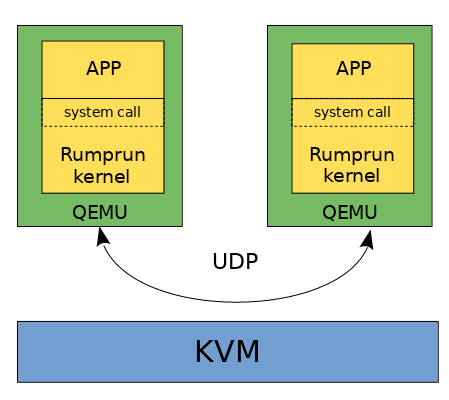
\includegraphics[scale=0.7]{figures/pipe_stage2.png}
%%\caption{Δεύτερο στάδιο υλοποίησης μηχανισμού pipe\label{fig4_3}}
%%\end{figure}
%%------------------------------------------------------------------------------
%%------------------------------------------------------------------------------

\subsubsection{Στάδιο 3 - pipe ως function call με shared memory}

Στο τελευταίο στάδιο, υλοποιήσαμε το μηχανισμό pipe, πάλι ως system call με τη
διαφορά ότι πλέον δε χρησιμοποιούνται sockets, αλλά κοινή μνήμη μεταξύ των
εικονικών μηχανημάτων. Πλέον δεν υπάρχει ανάγκη για ύπαρξη δικτύου μεταξύ των
εικονικών μηχανημάτων, ωστόσο η συγκεκιμένη υλοποίηση μπορεί να χρησιμοποιηθεί
μόνο για unikernels, που μοιράζονται τον ίδιο host. Για την κοινή μνήμη
χρησιμοποιήθηκε το ivshmem \cite{macdonell2011shared}. Όπως έχει ήδη αναφερθεί
πρόκειται για ένα μηχανισμό, που επιτρέεπει το διαμοιρασμό μνήμης μεταξύ του
host και των εικονικών μηχανών που εκτελούνται στο host. Η χρήση του γίνεται
μέσω μίας PCI συσκευής. Συνεπώς έπρεπε να δημιουργήσουμε τον κατάλληλο driver
που θα μας επιστρέψει να το χρησιμοποιήσουμε. Στην παρακάτω εικόνα \ref{fig4_4}
φαίνεται σχηματικά η υλοποίηση. 

\begin{figure}[htp]
\centering
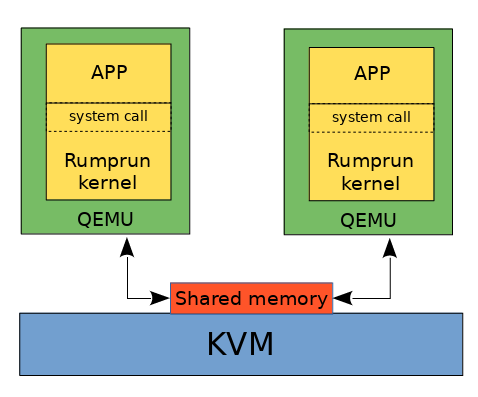
\includegraphics[scale=0.7]{figures/pipe_stage3.png}
\caption{Τρίτο στάδιο υλοποίησης μηχανισμού pipe\label{fig4_4}}
\end{figure}

Η χρήση του pipe, από την εφαρμογή γίνεται πλέον όπως σε κάθε UNIX λειτουργικό
σύστημα. Καλώντας την pipe, αν όλα πάνε καλά αποθηκεύονται στις
παραμέτρους fildes[0], fildes[1], οι δύο file descriptors που θα χρησιμοποιηθούν
για την ανάγνωση και εγγραφή αντίστοιχα. Σε περίπτωση επιτυχίας επιστρέφεται η
τιμή 0, ενώ σε αντίθετη περίπτωση, στη μεταβλητή errno αποθηκεύεται ο κωδικός
του σφάλματος. Επιπλέον έχουν υλοποιηθεί και όσα semantics δεν είχαν υλοποιηθεί
στα προηγούμενα στάδια. Οπότε, σε περίπτωση που δεν υπάρχουν ανοιχτά άκρα
ανάγνωσης στο pipe, η εγγραφή δε θα είναι επιτυχής. Αν δεν υπάρχει αρκετός χώρος
για την εγγραφή δεδομένων, τότε η write "μπλοκάρει".

Θα ξεκινήσουμε την περιγραφή της υλοποίησης από την υλοποίηση του PCI driver για
το ivshmem. Αρχικά πρέπει να ενημερώσουμε το qemu για τη χρήση του συγκεκριμένου
μηχανισμού. Για να γίνει αυτό χρησιμοποιούμε τις ακόλουθες παραμέτρους για το qemu.
\begin{lstlisting}[numbers=none]
-device ivshmem-plain,memdev=hostmem -object memory-backend-file,size=1M,share, mem-path=/dev/shm/ivshmem,id=hostmem
\end{lstlisting}
%% TODO na dw an isxuei auto pou grafw me to mempath
Στην παράμετρο size, ορίζουμε τη χωρητικότητα του pipe και για κάθε pipe πρέπει
να ορίσουμε διαφορετικό mem-path. Κάθε unikernel που ξεκινάει με τις
συγκεκριμένες παραμέτρους μπορεί να χρησιμοποιήσει το pipe. 

Από τη μεριά του unikernel, χρειάζεται να κατασκευάσουμε έναν PCI driver για το
μηχανισμό ivshmem. Όπως και στην περίπτωση του system call έτσι και στην
περίπτωση του driver, αρχικά πρέπει να φτιάξουμε το driver για το NetBSD. 
Ακολουθώντας το Kernel Development Manual του NetBSD ~\cite{NetBSDKDMDriver},
για τον pci device driver υλοποιήσαμε τρεις συναρτήσεις:
\begin{enumerate}
	\item match: Είναι η συνάρτηση που καλείται από το \EN{autoconfiguration}
		framework του NetBSD, όταν το σύστημα εκκινεί, ώστε να
		ταιριαστεί ο driver με τη συσκευή. Οπότε στην περίπτωση του
		δικού μας driver η συγκεκιμένη συνάρτηση ελέγχει αν πρόκειται
		για ivshmem pci device, ελέγχοντας τις τιμές του κατασκευαστή
		και το id της συσκευής.
	\item attach: Καλείται μόνο αν η ανίσχνευση της συσκευής ήταν επιτυχής
		(αν η match επέστρεψε 1). Ο ρόλος της είναι να αρχιοποιήσει τη
		συκευή. Δεδομένου, ότι εμείς χρησιμοποιούμε το συγκεκριμένο
		μηχανισμό απλά για διαμοιρασμό μνήμης, αρκεί να κάνουμε map το
		PCI\_BAR(2) του ivshmem και να αποθηκεύσουμε τις απαραίτητες
		μεταβλητές για τη χρήση του μηχανισμού.
	\item detach: Καλείται σε περίπτωση που η συσκευή αποσυνδεθεί. Στη δική
		μας περίπτωση είναι αρκετό να κάνουμε unmap το bus\_space που
		χρησιμοποιούμε και να μηδενίσουμε τις μεταβλητές που
		χρησιμοποιούμε για τη συσκευή.
\end{enumerate}

Προκειμένου να μπορεί να χρησιμοποιηθεί η συσκευή από τον υπόλοιπο πυρήνα του
NetBSD, είναι απαραίτητο να αποθηκευτούν οι απαραίτητες μεταβλητές που
αναφέρθηκαν στις συναρτήσεις attach και detach. Για το λόγο αυτό δημιουργήθηκε
το struct ivshm, που έχει ως πεδία τις μεταβλητές αυτές. 
\newpage
\begin{lstlisting}[numbers=none]
struct ivshm {
	bus_size_t		data_s;	/* size of shared memory */
	bus_addr_t		data_b;	/* base address of shared memory */
	bus_space_tag_t		data_t;	/* bus tag for shared memory */
	bus_space_handle_t	data_h;	/* bus handle for shared memory */
};
\end{lstlisting}
Ιδανικά θα θέλαμε να κάνουμε map όλη την κοινή μνήμη του ivshmem, ώστε να μπορεί
να χρησιμοποιηθεί σαν μνήμη του πυρήνα. Ωστόσο, το rumprun δεν υποστηρίζει το
maping μνήμης μέσω του bus. Ως εκ τούτου, η πρόσβαση στην κοινή μνήμη γίνεται
κάθε φορά με εγγραφή και ανάγνωση bytes από αυτήν χρησιμοποιώντας το bus. Υπό
αυτές τις συνθήκες, υπήρχαν τέσσερις μεταβλητές που ήταν απαραίτητες:
\begin{enumerate}
	\item το μέγεθος της κοινής μνήμης.
	\item η διεύθυνση βάσης της κοινής μνήμης
	\item το bus tag της κοινής μνήμης
	\item και το bus handle της κοινής μνήμης.
\end{enumerate}
Οι 2 τελευταίες μεταβλητές, είναι αυτές που χρησιμοποιούνται από τις συναρτήσεις
που παρέχει το NetBSD για να μπορέσει χρησιμοποιώντας το bus, να επικοινωνήσει
με τη συσκευή. Ο ρόλος των υπόλοιπων δύο μεταβλητών θα γίνει πιο ξεκάθαρος
παρακάτω.

Αφού λοιπόν, δημιουργήσαμε το driver για το NetBSD και ενημερώσαμε το
autoconfiguration framework για την ύπαρξη του, έπρεπε να κάνουμε γνωστή την
ύπαρξη του και στο rumprun. Για να γίνει αυτό απαιτούνται δύο ενέργεις. Πρώτον
προσθέτουμε το pci driver στο src-netbsd/sys/rump/dev/Makefile.rumpdevcomp.
Δεύτερον, να δημιουργηθεί ένα νέο directory στο src-netbsd/sys/rump/dev/lib/ για
τη νέα συσκευή. Το directory υατό περιέχει το ioconf και το απαραίτητο Makefile
για να προστεθεί o οδηγός μας στο build σύστημα του rumprun. 

\newpage
\begin{lstlisting}[caption={IVSHMEM.ioconf},captionpos=b]
ioconf ivshmem

include "conf/files"
include "dev/pci/files.pci"
include "rump/dev/files.rump"

pseudo-root pci*

ivshmem* at pci? dev ? function ?
\end{lstlisting}

\begin{lstlisting}[caption={rumprun Makefile για το ivshmem},captionpos=b]
RUMPTOP=${TOPRUMP}

.PATH:	${RUMPTOP}/../dev/pci

LIB=	rumpdev_ivshmem
COMMENT=ivshmem

IOCONF=	IVSHMEM.ioconf
RUMP_COMPONENT=ioconf

SRCS+=	ivshmem.c
##SRCS+=	ivshmem_component.c

CPPFLAGS+= -I${RUMPTOP}/librump/rumpkern

.include "${RUMPTOP}/Makefile.rump"
.include <bsd.lib.mk>
.include <bsd.klinks.mk>
\end{lstlisting}

Η αρθρωτή οργάνωση των unikernels, δίνει τη δυνατότητα κάθε φορά να επιλέγονται
μόνο τα απαραίτητα συστατικά για κάθε unikernel. Σε αυτό αποσκοπεί και η
δημιουργία του παραπάνω directory, ώστε να μπορεί ο συγκεκιμένος driver να
ενσωματωθεί στο unikernel, κατά τη διάρκεια του baking. Για τη χρήση του
συγκεκριμένου οδηγού είναι απαραίτητη η εισαγωγή του -lrumpdev\_ivshmem στο
config με το οποίο θα γίνει bake η εφαρμογή. 

Αφού δημιουργήσαμε τον driver, το επόμενο βήμα ήταν η αλλαγή του system call,
ώστε αντί για sockets να χρησιμοποιείται ο μηχανισμός του ivshmem. Αρχικά, δε
χρειαζόμαστε την ioctl κλήση και δημιουργούμε δύο structs, το struct pipe και το
struct pipe\_op. Οι ορισμοί τους φαίνονται παρακάτω:

\begin{lstlisting}
struct pipe {
	bus_size_t	init;		/* is shared memory initalized? */
	bus_size_t	lock;		/* pipe lock */
	bus_size_t	wr_lock;	/* writers lock */
	bus_size_t	nreaders;	/* number of readers in pipe */
	bus_size_t	nwriters;	/* number of writers in pipe */
	bus_size_t	len;		/* size of pipe buffer */
	bus_size_t	in;		/* pointer for next write */
	bus_size_t	out;		/* pointer for next read */
	bus_size_t	cnt;		/* number of bytes in pipe */
	bus_size_t	buf;		/* pipe buffer */
	int		pr_readers;	/* readers from this process */
	int		pr_writers;	/* writers from curr process */
};

struct pipe_op {
	int		oper;		/* operation in pipe 0 for read,
					   1 for write*/
	struct pipe	*pipe;
};
\end{lstlisting}

Το struct pipe\_op συνδέεται με τα file descriptors που δημιουργεί η κλήση pipe,
ένα για κάθε file descriptor. H μεταβλητή oper, καθορίζει αν πρόκειται για το
file descriptor που αφορά την εγγραφή στο pipe ή αυτό που αφορά στην ανάγνωση. η
άλλη τιμή είναι το struct pipe που είναι κοινό και για τα δύο άκρα του pipe και
περιέχει βοηθητικές μεταβλητές για τη διαχείρηση του pipe. Όπως έχει ήδη
αναφερθεί η χρήση της κοινής μνήμης γίνεται μέσω του bus και οι συναρτήσεις
εγγραφής ή ανάγνωσης από το bus απαιτούν ως παράμετρο τη διεύθυνση βάσης από την
οποία θα διαβαστούν τα δεδομένα. Έτσι για να αναφερθούμε σε διαφορετική
μεταβλητή μέσα σε αυτή τη μνήμη θα πρέπει να χρησιμοποιήσουμε διαφορετική
διεύθυνση βάσης. Συνεπώς, το struct pipe περιέχει τις διευθύνσεις των κοινών
μεταβλητών στην κοινή μνήμη. Επιπλέον, χρησιμοποιούνται και οι μεταβλητές
pr\_readers και pr\_writers που αφορούν τα ανοιχτά άκρα στο pipe από τη
συγκεκριμένη διεργασία. Η δύο τελευταίες μεταβλητές είναι απαραίτητες για τη
διαχείρηση του pipe όταν η διεργασία που έχει δημιουργήσει το pipe κάνει fork.

\begin{figure}[htp]
\centering
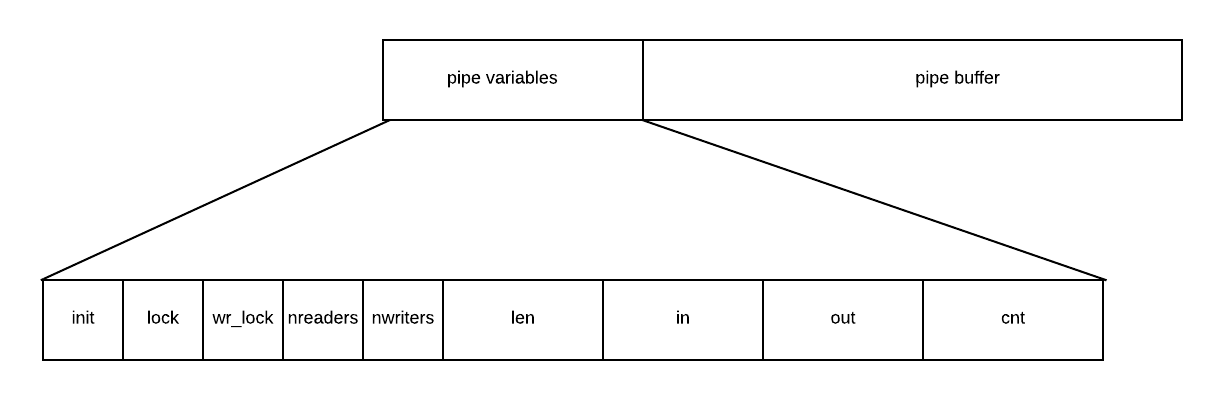
\includegraphics[scale=0.7]{figures/shared_memoery_layout.png}
\caption{shared memory layout\label{fig4_5}}
\end{figure}

Αν θεωρήσουμε την κοινή μνήμη σαν ένα μεγάλο συνεχόμενο κομμάτι μνήμης, τότε
στην παραπάνω εικόνα ~\ref{fig4_5} φαίνεται πως την έχουμε διαχωρίσει εσωτερικά,
με ένα κομμάτι της να αφορά τις μοιραζόμενες μεταβλητές και ένα άλλο τον buffer
του pipe. Οι αρχικές μεταβλητές, έχουν μικρότερο μέγεθος από τις τελευταίες και
η λειτουργία της κάθε μίας έχει ώς εξής:
\begin{itemize}
	\item init: Πρόκειται για μία μεταβλητή ελέγχου, που καθορίζει αν έχουν
		αρχικοποιηθεί οι κοινές μεταβλητές του pipe. Αλλάζεις μόνο δύο
		φορές, όταν πρωτοδημιουργείται το pipe και όταν αυτό
		καταστρέφεται. Ουσιαστικά δηλώνει αν οι υπόλοιπες μεταβλητές
		περιέχουν "σκουπίδια", ή αν έχουν χρήσιμες τιμές.
	\item lock: Πρόκειται για το γενικό lock του pipe και προστατεύει όλες
		τις κοινές μεταβλητές του pipe. 
	\item wr\_lock: Πρόκειται για ένα lock που κάθε φορά επιτρέπει σε ένα
		και μόνο unikernel ννα γράφει στο pipe. 
	\item nreaders: Ο αριθμός των ανοιχτών άκρων ανάγνωσης για το pipe
	\item wreaders: Ο αριθμός των ανοιχτών άκρων εγγραφής για το pipe
	\item len: Το μέγεθος του pipe buffer.
	\item in: Ο δείκτης που καθορίζει σε ποιο σημείο θα γραφτούν τα νέα
		δεδομένα στο pipe buffer.
	\item out: Ο δείτης που καθορίζει από ποιο σημείο θα διβαστούν δεδομένα
		από το pipe buffer
	\item cnt: Μετρητής των bytes που υπάρχουν στο pipe, κάθε στιγμή
\end{itemize}

Για την πρόσβαση στις παραπάνω μεταβλητές και γενικά για την κοινή μνήμη
χρησιμοποιήθηκαν οι συναρτήσεις bus\_space\_read\_1, bus\_space\_read\_4,
bus\_space\_write\_1, bus\_space\_write\_4. Ο αριθμός στο τέλος της κάθε
συνάρτησης υποδηλώνει το μέγεθος των δεδομένων που θα διαβαστούν ή θα γραφτούν.
Για την πιο εύκολη χρήση της κοινής μνήμης δημιουργήθηκαν 4 βοηθητικές
συναρτήσεις, που φαίνονται παρακάτω. 

\begin{lstlisting}
/*
 * Read a region of bytes in bus (data is 1 byte)
 */
void read_region_1(bus_size_t offset, uint8_t *datap, bus_size_t count)
{
	int i;
	for (i=0; i<count; i++) {
		datap[i] = bus_space_read_1(sharme.data_t, sharme.data_h,
				offset + i);
	}
	return;
}

/*
 * Read a region of bytes in bus (data is 4 byte)
 */
void read_region_4(bus_size_t offset, uint32_t *datap, bus_size_t count)
{
	int i;
	for (i=0; i<count; i++) {
		datap[i] = bus_space_read_4(sharme.data_t, sharme.data_h,
				offset + i*4);
	}
	return;
}

/*
 * Write in a region of bytes in bus (data is 1 byte)
 */
void write_region_1(bus_size_t offset, uint8_t *datap, bus_size_t count)
{
	int i;
	for (i=0; i<count; i++) {
		bus_space_write_1(sharme.data_t, sharme.data_h, offset + i,
				datap[i]);
	}
	return;
}

/*
 * Write in a region of bytes in bus (data is 4 byte)
 */
void write_region_4(bus_size_t offset, uint32_t *datap, bus_size_t count)
{
	int i;
	for (i=0; i<count; i++) {
		bus_space_write_4(sharme.data_t, sharme.data_h,	offset + i*4,
				datap[i]);
	}
	return;
}
\end{lstlisting}

Οι παραπάνω συναρτήσεις διαβάζουν ή γράφουν σε μία περιοχή μνήμης, είτε 1 είτε 4
bytes δεδομένα. Το μέγεθος της περιοχής που θα γίνει η πρόσβαση καθορίζεται από
την παράμετρο count και το μέγεθος των bytes (count * bytes\_of\_data). Οι άλλες
2 παράμετροι των συναρτήσεων είναι η διεύθυνση βάσης για το bus και ένας πίνακας
, στον οποίο αποθηκεύονται τα δεδομένα που διαβάστηκαν από μνήμη είτε τα
δεδομένα που θα γραφτούν στην περίπτωση, στις λειτουργίες read και write
αντίστοιχα. Οι συναρτήσεις bus\_space, χρησιμοποιούν τη δομή struct ivshm, για
τις μεταβλητές bus tag και bus handle. Όλες οι αναφορές στην κοινή μνήμη, πέρα
από αυτές των locks, γίνονται χρησιμοποιώντας αυτές τις συναρτήσεις.

Η ύπαρξη κοινής μνήμης μεταξύ διαφορετικών unikernels, απαιτεί και την ύπαρξη
κάποιου συγχρονισμού μεταξύ αυτών. Για αυτό σκοπό χρησιμοποιούνται τα δύο locks
στο struct pipe (lock, wr\_lock). Τα δύο αυτά locks, βρίσκονται εντός της κοινής
μνήμης και απαιτούν ειδική μεταχείριση. Ο μηχανισμός ivshmem μπορεί να
υποστηρίξει τη χρήση ατομικών εντολών του gcc. Για το λόγο, αυτό δημιουργήσαμε
δύο ακόμα συναρτήσεις για το locking, μία για την απόκτηση του κλειδώματος και
μία για την απελευθέρωση του. Ου συναρτήσεις αυτές φαίνονται παρακάτω. 

\begin{lstlisting}
/*
 * Spinlock for pipe
 */
void pipe_lock(bus_size_t lock)
{
	while(__sync_val_compare_and_swap((uint8_t *)sharme.data_b + lock, 0, 1) == 1)
		/* do nothing */;
	return;
}

/*
 * Release the lock
 */
void pipe_unlock(bus_size_t lock)
{
	__sync_lock_release((uint8_t *)sharme.data_b + lock);
	return;
}

\end{lstlisting}

Οι ατομικές εντολές που χρησιμοποιήθηκαν για τη χρήση του lock, είναι οι
\_\_sync\_val\_compare\_and\_swap και \_\_sync\_lock\_release. Οι εντολές αυτές
δέχονται ως παράμετρο τη διεύθυνση της μνήμης στην οποία θα γίνει η πρόσβαση. Η
διεύθυνση αυτή καθορίζεται από τη διεύθυνση βασης των δεδομένων (data\_b) στο
struct ivshmem και το offset του lock μέσα στην κοινή μνήη που είναι
αποθηκευμένο στο struct pipe. Οποιαδήποτε αλλαγή σε κάποιο κομμάτι της κοινή
μνήμης απαιτεί την απόκτηση του γενικού lock, ενώ οποιαδήποτε εγγραφή στο pipe
θα πρέπει να έχει πάρει τον έλεγχο του wr\_lock.

Όταν λοιπόν, η εφαρμογή που εκτελείται σε ένα unikernel εκτελέσει την κλήση
pipe, από τη μεριά του πυρήνα πέρα από τη δημιουργία των file descriptors και τη
σύνσεση τους με το εκάστοτε struct pipe\_op συμβαίνουν τα εξής. Αρχικά,
δημιουργείται το struct pipe και αρχικοποιούνται όλες οι μεταβλητές τους με το
offset της κάθε μίας στην κοινή μνήμη. Ύστερα, ξεκινά ο έλεγχος της κοινής
μνήμης. Ελέγχεται η τιμή της init στην κοινή μνήμη και ανάλογα με την τιμή της η
κοινή μνήμη, είτε θα αρχικοποιειθεί είτε όχι. Στη συνέχεια, αφού η περιοχή
μνήμης έχει αρχικοποιηθεί, αυξάνονται οι μετρητές των άκρων του pipe και τέλος
συνδέεται το κοινό struct pipe με τα struct pipe\_op. Η κλήση επιστρέφει τους
file descriptors στην εφαρμογής και το pipe είναι πλέον έτοιμο να
χρησιμοποιηθεί. Ειδική σημείωση πρέπει να γίνει για τον έλεγχο της τιμής init
στην κοινή μνήμη. Η κοινή μνήμη πρέπει να καταστραφεί, αν δεν υπάρχουν pipes που
τη χρησιμοποιούν καθώς σε διαφορετική περίπτωση μπορεί λόγω του τρόπου ελέγχου
της init, να μην αρχικοποιηθεί. 

Σημαντικό ρόλο στον παραπάνω σκοπό έχει η κλήση close σε ένα file descriptor του
pipe. Στην απλή περίπτωση που δεν πρόκειται για το τελευταίο file descriptor του
pipe, απλά ενημερωονται οι μετρητές των ανοιχτών άκρων του pipe. Αν όμως,
πρόκειται να κλείσει το τελευταίο file descriptor που αφορά το συγκεκριμένο pipe
τότε μηδενίζεται όλη η κοινή μνήμη που χρησιμοποιήθηκε. Με αυτό τον τρόπο την
επόμενη φορά που θα χρησιμοποιηθεί το συγκεκριμένο κομμάτι μνήμης η τιμή init θα
υποδηλώνει ότι πρέπει η κοινή μνήμη να αρχικοποιηθεί. 

\begin{figure}[htp]
\centering
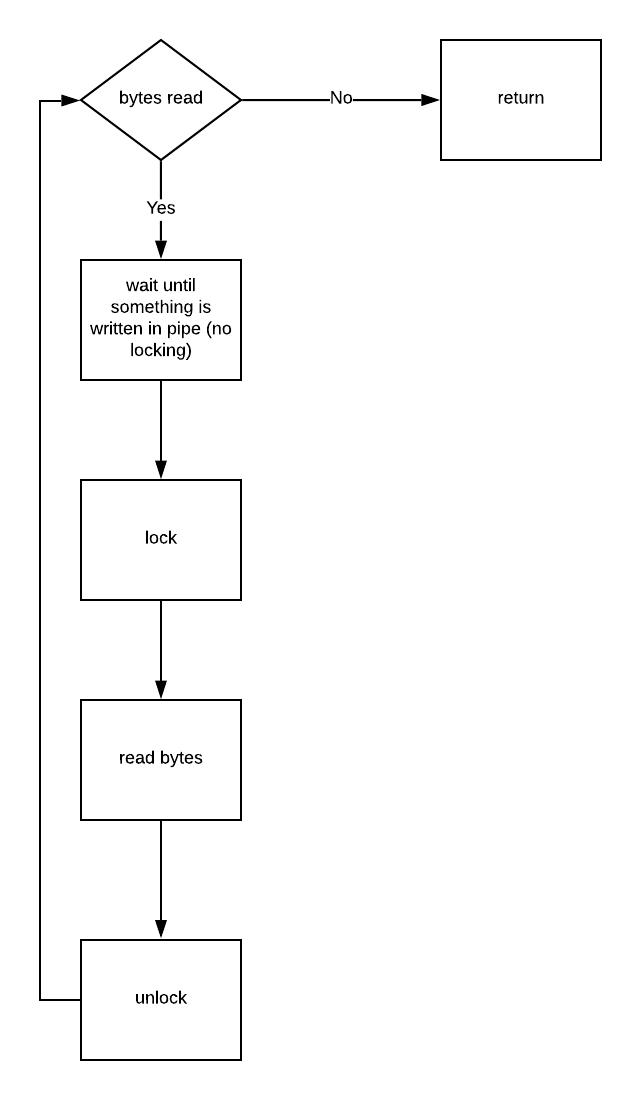
\includegraphics[scale=0.7]{figures/pipe_read.png}
\caption{pipe read flow chart\label{fig4_6}}
\end{figure}

Στην παραπάνω εικόνα ~\ref{fig4_6} φαίνεται το διάγραμμα ροής, όταν εκτελείται η
κλήση read σε άκρο ανάγνωσης του pipe. Ουσιαστικά πρόκειται για ένα while loop,
το οποίο τερματίζει υπό τέσσερις ορισμένες συνθήκες:
\begin{enumerate}
	\item Αν έχουν διαβαστεί όσα bytes ζήτησε η εφαρμογή
	\item Αν έχουν διαβαστεί όλα τα bytes από το pipe (ανεξάρτητα από τα
		πόσα ζήτησε η εφαρμογή) 
	\item Αν δεν υπάρχουν δεδομένα να διαβαστούν και όλα τα άκρα εγγραφής
		έχουν κλείσει
	\item Αν κάτι πάει στραβά κατά τη διαδικασία μεταφοράς δεδομένων από την
		κοινή μνήμη στην εφαρμογή.
\end{enumerate}
Για την αποφυγή deadlocks, αρχικά γίνεται έλεγχος για τη διαθεσιμότητα δεδομένων
στο pipe χωρίς την απόκτηση του γενικού κλειδώματος. Σε περίπτωση, που υπάρχουν
δεδομένα, τότε αποκτάται το κλείδωμα και επαναλαμβάνεται ο έλεγχος με την κατοχή
του κλειδώματος. Αφού λοιπόν μεταφερθύν τα δεδομένα από την κοινή μνήμη στην
εφαρμογή, τότε ενημερώνονται οι κοινές μεταβλητές του pipe (out, cnt) και
ελευθερώνεται το lock. Καθώς ο buffer του pipe είναι κυκλικός, πρέπει να
λαμβάνουμε υπόψιν την περίπτωση που έχουμε φτάσει στο τέλος του buffer, οπότε
πρέπει να ξεκινήσουμε να διαβάζουμε τα υπόλοιπα δεδομένα από την αρχή. Τέλος,
τόσο κατά τη διάρκεια του ελέγχου δεδομένων χωρίς αλλά και με το κλείδωμα,
ελέγχονται και τα ανοιχτά άκρα εγγραφής στο pipe. Αν όλα έχουν κλείσει τότε
πρέπει να επιστρέψει η κλήση pipe καθώς δεν πρόκειται να εγγραφούν νέα δεδομένα.

\begin{figure}[htp]
\centering
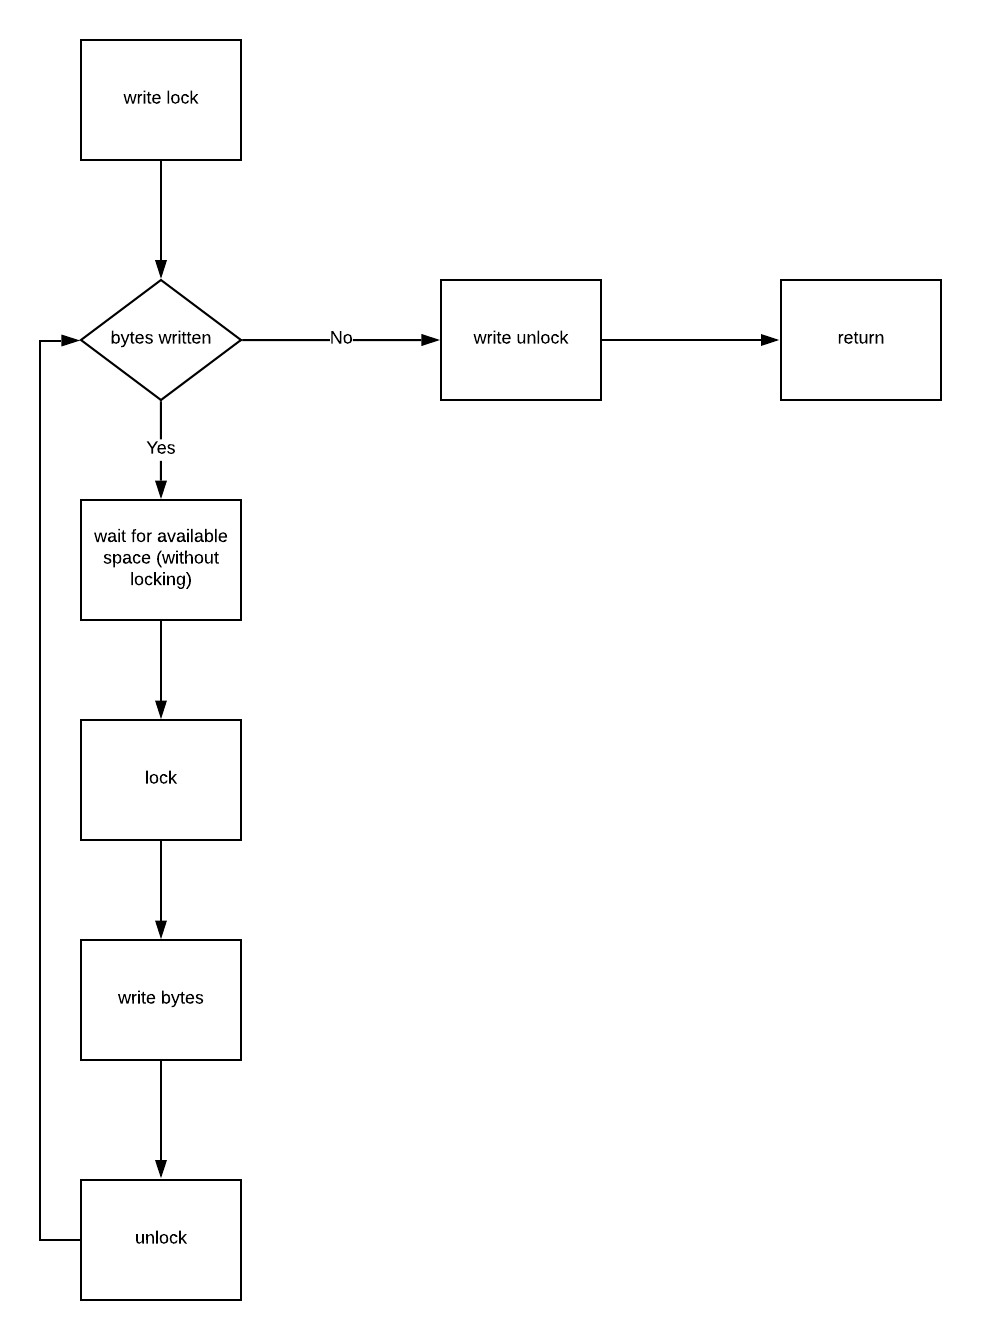
\includegraphics[scale=0.7]{figures/pipe_write.png}
\caption{pipe write flow chart\label{fig4_7}}
\end{figure}

Στην παραπάνω εικόνα ~\ref{fig4_7} φαίνεται το διάγραμμα ροής της κλήσης write
του pipe. Όπως φαίνεται δεν έχει κάποια ιδιαίτερη διαφορά με το διάγραμμα ροής
της κλήσης read, εκτός από το γεγονός ότι από την αρχή μέχρι το τέλος της
εκτέλεσης της δεσμεύεται το wr\_lock. Ο λόγος ύπαρξης ενός τέτοιου κλειδώματος,
είναι για να επιτευχθεί η ατομικότητα της κλήσης write σε ένα pipe. Από εκεί και
πέρα, όπως και πριν αρχικά ελέγχουμε αν υπάρχει διαθέσιμος χώρος στην κοινή
μνήμη για την εισαγωγή νέων δεδομένων. Έπειτα αποκτάται το κλείδωμα και
επαναλαμβάνεται ο έλεγχος διαθέσιμου χώρου. Αν είναι επιτυχής, γίνεται η εγγραφή
δεδομένων στην κοινή μνήμη και ενημερώνονται οι αντίστοιχες μεταβλητές (in,
cnt). Καθώς οbuffer του pipe είναι κυκλικός πρέπει να λαμβάνουμε υπόψιν την
περίπτωση που ο διαθέσιμος χώρος βρίσκεται την αρχή του buffer. Τόσο κατά τη
διαδικασία ελέγχου διαθέσιμου χώρου χωρίσς κλείδωμα όσο και με κλείδωμα,
ελέγχονται και τα ανοιχτά άκρας ανάγνωσης του pipe. Αν όλα έχουν κλείσει τότε
πρέπει να επιστρέψει η κλήση pipe με το error EPIPE, καθώς δεν υπάρχουν
αναγνώστες να διαβάσουν τα δεδομένα. Τέλος, ´ολα τα παραπάνω βρίσκονται μέσα σε
ένα while loop το οποίο μπορεί να τερματίσει υπό τις τέσσερις παρακάτω συνθήκες.
\begin{enumerate}
	\item Αν έχουν γραφτεί όσα bytes ζήτησε η εφαρμογή
	\item Αν δεν υπάρχει κανένα ανοιχτό άκρο ανάγνωσης στο pipe.
	\item Αν κάτι πάει στραβά κατά τη διαδικασία μεταφοράς δεδομένων από την
		την εφαρμογή στην κοινή μνήμη.
\end{enumerate}

\newpage
\section{Μηχανισμός fork}

Η κλήση fork δημιουργεί μία νέα διεργασία (παιδί), η οποία είναι όμοια με τη
διεργασία που την κάλεσε (γονέας). Και στις δύο διεργασίες ο κώδικας θα
συνεχίσει να εκετελείται μετά την κλήση της fork. Στη διεργασία γονέας, η κλήση
επιστρέφει το process id του παιδιού, ενώ στη διεργασία παιδί επιστρέφει 0.
Αντιθέτως αν έχει υπάρξει κάποιο πρόβλημα κατά την κλήση της τότε επιστρέφεται η
τιμή -1 και ο κωδικός του σφάλματος αποθηκεύεται στη μεταβλητή errno. Η
διεργασία παιδί υιοθετεί από τη διεργασία γονέα τα file descriptors. Μία
συνηθισμένη πρακτική είναι να δημιουργούνται διεργασίες παιδιά τα οποία εκτελούν
συγκεκριμένες ενέργειες και επικοινωνούν με το γονέα μέσω διαδεργασιακής
επικοινωνίας όπως pipe. Ένα εξίσου συχνό φαινόμενο είναι οι διεργασίες παιδιά να
εκτελούν μία διαφορετική εφαρμογή, κάνοντας χρήση μίας exec κλήσης. 

Οι παραπάνω λειτουργίες υλοποιούνται στα περισσότερα συμβατικά λειτουργικά
συστήματα αλλά όχι στα unikernel frameworks, μέχρι τη στιγμή εγγραφής αυτής της
εργασίας. Εξαίρεση αποτελεί το library operating system Graphene
~\cite{tsai2014cooperation} που επιτρέπει την εκτέλεση multi-process εφαρμογών.
Τα περισσότερα unikernel frameworks, στοχεύουν στη δημιουργία unikernels που
εκτελούν μία και μόνο εφαρμογή, ως μία διεργασία. Προσπαθώντας να κρατήσουμε
αυτό το βασικό χαρακτηριστικό τους σχεδιάσαμε και υλοποιήσαμε ένα μηχανισμό
fork, που δίνει τη δυνατότηταότητα σε unikernels να μπορούν να χρησιμοποιήσουν
τη συγκεκριμένη κλήση. Η διαφορά είναι ότι η νέα διεργασία δε θα δημιουργηθεί
μέσα στο υπάρχον unikernel, αλλά θα δημιουργηθεί ένα νέο unikernel όμοιο με το
αρχικό. Αφαιρετικά θεωρούμε κάθε unikernel ως μία διεργασία και το hypervisor,
ως το λειτουργικό σύστημα που θα δημιουργήσει και θα διαχειριστεί τις διεργασίες
- εικονικές μηχανές. Η υλοποίηση, δεν παρέχει όσες δυνατότητες θα παρείχε ένα
συμβατικό λειτουργικό συτημα, παρά μόνο τη δημιουργία μίας νέας οικονικής
μηχανής που μπορεί να επικοινωνεί με το γονέα μέσω του μηχανσιμού pipe, που
αναλύθηκε προηγουμένως. Σε αυτή την περίπτωση, θα πρέπει να προστεθεί η παράμετρος master=on στην επιλογή device του ivshmem-plain.

Η υλοποίηση έγινε για το Rumprun, πάνω από το QEMU/KVM (συγκεκριμένα την έκδοση
2.11.2 https://download.qemu.org/qemu-2.11.2.tar.xz), ωστόσο οποιοδήποτε
unikernel framework, μπορεί να εκτελεστεί στο QEMU/KVM μπορεί να χρησιμοποιήσει
το συγκεκριμένο μηχανισμό. Σε γενικές γραμμές, όταν μία εφαμρογή κάνει χρήση της
κλήσης fork, σε ένα unikernel αυτή η κλήση μετατρέπεται σε hypercall από τον
πυρήνα του Rumprun προς το QEMU/KVM. Στη συνέχεια το QEMU?KVM είναι αυτό που
ξεκινά τη διαδικασία δημιουργίας μίας νέας εικονικής μηχανής, η οποία είναι ίδια
με την αρχική (γονέα). Όταν δημιουργηθεί αυτή η εικονική μηχανή, επιστρέφεται ο
έλεγχος στην εικονική μηχανή γονέα, η οποία πλέον μπορεί να συνεχίσει την
εκτέλεση της. 

Στην παρακάτω εικόνα \ref{fig4_8}, φαίνεται όλη η διαδικασία, από τη στιγμή [πυ
μία εφαρμογή καλεί την fork, μέχρι να επιστρέψει ο έλεγχος σε αυτή. Έπειτα
ακολουθεί η αναλυτική περιγραφή του μηχανισμού, δίνοντας ιδιαίτερη έμφαση στα
σημαντικά σημεία. Η περιγραφή θα ξεκινήσει από την εφαρμογή που καλεί την fork
και θα συνεχίζει βήμα βήμα. Η διαδικασία εισαγωγής κλήσης συστήματος στο Rumprun
δε θα αναλυθεί, καθώς αυτό έχει γίνει ήδη στην περίπτωση του μηχανσιμού pipe.

\begin{figure}[htp]
\centerline{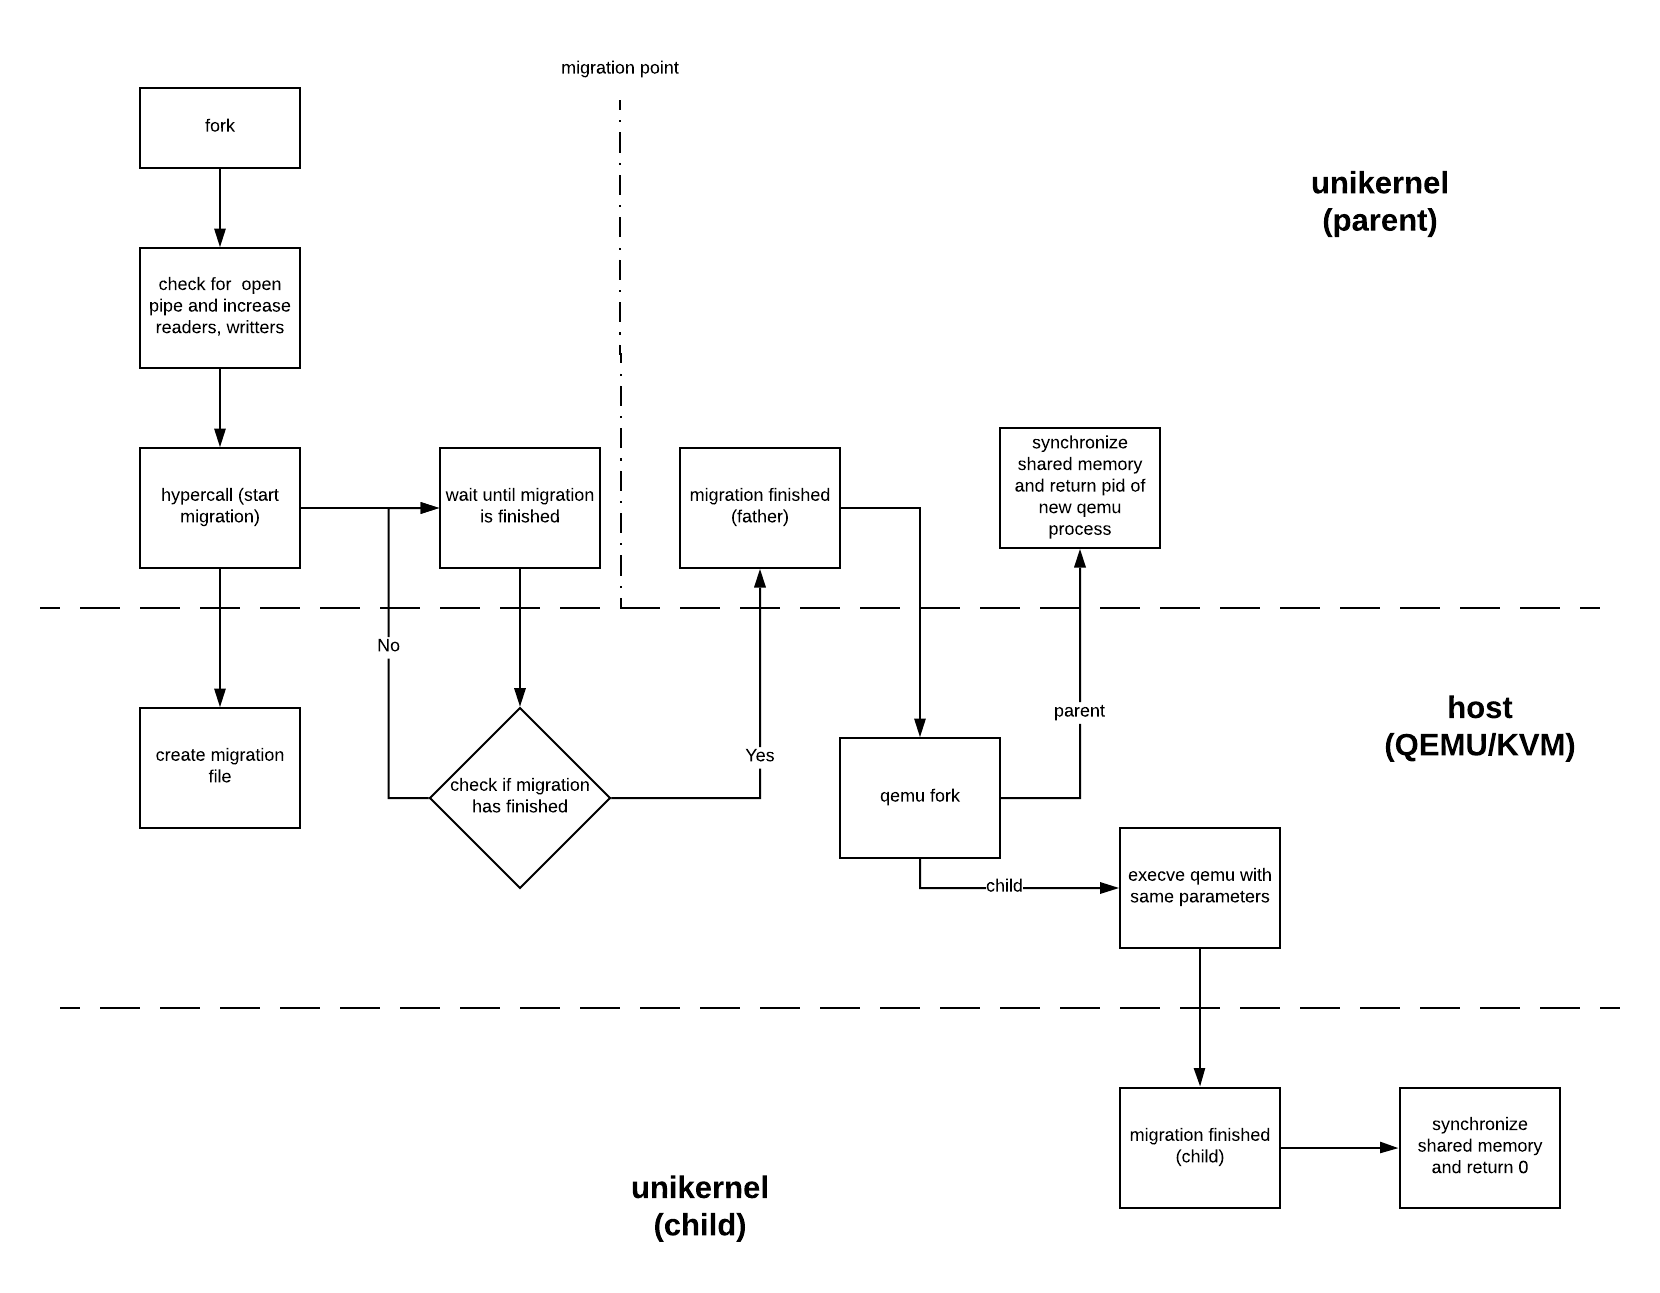
\includegraphics[scale=0.7]{figures/fork_olo.png}}
\caption{fork flow chart\label{fig4_8}}
\end{figure}

\subsection{Ενημέρωση του pipe}
Το πρώτο πράγμα που πρέπει να γίνει από την κλήση συστήματος, είναι ο έλεγχος αν
υπάρχει ανοιχτό pipe, από την εφαρμογή που καλεί την fork. Όπως έχουμε αναφέρει
παραπάνω, αποτελεί συχνό φαινόμενο η δημιουργία ενός pipe πριν την κλήση fork,
ώστε να μπορούν οι δύο διεργασίες (γονιός, παιδί) να επικοινωνούν χρηιμοποιώντας
το pipe που χει δημιουργήσει ο γονέας. Δεδομένου ότι πρόκειται για ένα νέο
μηχανσιμό pipe, θα πρέπει να εκτελεστούν οι ανάλογες ενέργεις για τη σωστή
διαχείρηση του. Όπως και σε ένα συμβατικό λειτουργικό συτημα η διεργασία παιδί
υιοθετεί τα ανοιχτά file descriptors της διεργασίας γονέας. Στη δικιά μας
περίπτωση, αφού έχουμε εικονικές μηχανές και η εικονική μηχανή παιδί είναι
κλώνος αυτής του γονέα. Έτσι, γνωρίζουμε ότι θα διατηρηθουν τα file descriptors
και στο unikernel παιδί. Συνεπώς, απομένει μία μόνο ενέργεια, να ενημερώσουμε το
pipe για την ύπαρξη περισσότερων ανοιχτών και κλειστών άκρων. 

Ο τρόπος με τον οποίο γίνεται ο έλεγχος για την ύπαρξη ανοιχτού pipe γίνεται,
ελέγχοντας τα file descriptors της εφαρμογής. Ελέγχοντας, λοιπόν, όλα τα file
descriptors της εφαρμογής, βρίσκουμε αν υπάρχουν file descriptors για το δικό
μας μηχανισμό pipe. Από τη στιγμή που βρεθεί κάποιο, θα πρέπει να ενημερώσουμε
το pipe ότι θα αυξηθούν τα ανοιχτά άκρα ανάγνωσης και εγγραφής σε αυτό.
Χρησιμοποιώντας τη δομή file\_t, στην οποία αποθηκεύει ο πυρήνας του NetBSD τα
απαραίτητα στοιχεία του file descriptor, μπορούμε να αποκτήσουμε πρόσβαση στη
δομή struct pipe\_op και κατε επέκταση στη δομή struct pipe του μηχανσιμού pipe.
Η δομή pipe\_op, μας πληροφορεί για το αν πρόκειται για άκρο εγγραφής ή για άκρο
ανάγνωσης στο pipe. Χρησιμοποιώντας τη δομή pipe, μπορούμε να χρησιμοποιήσουμε
την κοινή μνήμη και να ενημερώσουμε τις αντίστοιχες μεταβλητές. Η ενημέρωση
γίνεται φυσικά, δεσμεύοντας το γενικό lock του pipe και αυξάνοντας κατά ένα τις
μεταβλητές nreaders και nwriters, αν το άκρο ανάγνωσης είναι ανοιχτό ή το άκρο
εγγραφής είναι ανοιχτό αντίστοιχα. 

Από τη μεριά του pipe δε χρειάζεται να πειράξουμε κάτι άλλο. Η εικονική μηχανή
παιδί, όντας κλώνος της εικονικής μηχανής γονέα θα έχει πρόσβαση στην
μοιραζόμενη μνήμη. Αν δεν υπάρχει κάποιο pipe από το unikernel γονέα, τότε καμία
ενέργεια δε συμβαίνει στο παρών στάδιο.

\subsection{Hypercall εκκίνησης migration}

Από αυτό το στάδιο ξεκινάει η διαδικασία για τη δημιουργία μία εικονικής μηχανής
που θα ναι κλώνος με την αρχική. Την κλωνοποίηση και την εκκίνηση της νέας
εικονικής μηχανής αναλαμβάνει εξ' ολοκλήρου το QEMU/KVM. Από τη μεριά του τo 
unikernel, περιμένει την ολοκλήρωση αυτή της διαδικασίας, χωρίς να επιστρέφει
τον έλεγχο στην εφαρμογή, αλλά παραμένοντας εντός του πυρήνα. Με λίγα λόγια, η
διαδικασία κλωνοποίησης της εικονικής μηχανής - γονέα, γίνεται χρησιμοποιώντας
τους μηχανισμούς migration που προσφέρει το QEMU. 

Με βάση αυτά τα δεδομένα, το πρώτο στάδιο για τη δημιουργία της εικονικής
μηχανής - παιδί είναι η δημιουργία του migration file, με βάση το οποίο θα
εκκινήσει αργότερα το QEMU, τη νέα εικονική μηχανή. Όλη η επικοινωνία μεταξύ του
unikernel και του QEMU, γίνεται μέσω hypercalls. Δεδομένου, ότι απαιτείται η
μεταφορά κάποιων δεδομένων από το QEMU στο unikernel, τα hypercalls αυτά είναι
στην ουσία vm exits, που γίνονται χρησιμοποιοώντας την εντολή in, της assembly
σε κάποιο συγκεκριμένο I/O port. 

Για την εκκίνηση του migration το unikernel εκτελεί το hypercall, που ζητά
δεδομένα από το I/O port 0x77dd. Αυτό έχει ως αποτέλεσμα, να γίνει vm exit και ο
έλεγχος να βρίσκεται πλέον στην πλευρά του QEMU. Το unikernel αναμένει να λάβει
απάντηση από το I/O port, την οποία απάντηση θα δώσει το QEMU. Από τη μεριά του
QEMU, αφού διαπιστωθεί ότι πρόκειται για το συγκεκριμένο vm exit, ξεκινάει τη
διαδικασία του migration και επιστρέφει την τιμή 0 στο unikernel. H συγκεκριμένη
τιμή απλά υποδηλώνει στο unikernel, ότι έχει ξεκινήσει η διαδικασία δημιουργίας
του migration file. Η τοποθεσία του migration file, είναι προκαθορισμένη και
είναι η εξής /tmp/vm\_migration.out. 

Η δημιουργία του migration file, γίνεται με τον ίδιο τρόπο που εκτελεί τη
συγκεκριμένη λειττουργία το QEMU, όταν του δοθεί η συγκεκριμένη εντολή. Δηλαδή,
χρησιμοποιείται ο ίδιος ο μηχανσιμός του QEMU, με μία μικρή αλλαγή. Το QEMU,
αφού περατώσει τη διαδικασία του migration, σταματά την αρχική εικονική μηχανή.
Από τη δικιά μας μεριά, αυτό δεν είναι επιθυμητό αφού το unikernel γονέας,
θέλουμε να μπορεί να συνεχίσει την εκτέλεση του. Συνεπώς, απαιτούνται κάποιες
αλλαγές στον κώδικα του migration από το QEMU, ώστε μετά το πέρας του migration,
να μην σταματά η εκτέλεση της αρχικής εικονικής μηχανής. Για την υλοποίηση,
αυτής της αλλαγής, αφού έχει ολοκληρωθεί η δημιουργία του migration file, πριν
επιστρέψει η συνάρτηση που χειρίζεται το migration, καλείται η qmp\_cont, η
οποία ξαναεκκινεί την εικονική μηχανή. Η συγκεκριμένη συνάρτηση, καλείται από το
QEMU, όταν του δοθεί η εντολή να συνεχίσει τη λειτουργία, μία εικονικής μηχανής
της οποίας η λειτουργεία έχει παύσει. 

Εν κατακλείδι, η διαδικασία της δημιουργίας του migration file, γίνεται
χρησιμοποιώντας τις λειτουργίες που προσφέρει ήδη το QEMU. Ωστόσο, για να μην
αλλοιωθεί η κανονική λειτουργία του migration, από την αλλαγή που προσθέσαμε,
αντιγράψαμε τον αρχικό κώδικα και προσθεσαμε στο νέο αντίγραφο την παραπάνω
αλλαγή. Με αυτό τον τρόπο, διατηρείται ηαρχική μορφή του migration από το QEMU
και ικανοποιούμε την απαίτηση, η εικονική μηχανή γονέας να συνεχίζει την
εκτέλεση της. 

\subsection{Hypercall ελέγχου migration}

Ο τρόπος με τον οποίο εκτελεί το QEMU τη διαδικασία του \EN{migration}, είναι
δημιουργώντας ένα νήμα, που έχει ένα και μόνο ρόλο, να φέρει εις πέρας την όλη
διδικασία του migration. Επιπλέον είναι αναγκαίο η εικνοική μηχανή να εκτελείται
κατά τη διάρκεια του migration. Προκειμένου να ενημερωθεί ο πυρήνας του Rumprun
για το τέλος της διαδικασίας του migration, αλλά και να εκτελείται η εικονική
μηχανή, χρησιμοποιούμε ένα δεύτερο hypercall. Όπως και πριν το hypercall
υλοποιείται με vm exit για Ι/Ο request, αλλά στη θύρα 0x77db αυτή τη φορά. 

Αφού, λοιπόν, ξεκινήσει η διαδικασία του migration και δοθεί ο έλεγχος στην
εικονική μηχανή, εκείνη παραμένοντας μέσα στο system call της fork, περιμένει
την ολοκλήρωση του migration. Η αναμονή αυτή έχει υλοποιηθεί με busy wait,
χρησιμοποιοώντας ένα loop που κάνει συνεχώς hypercalls, γιανα ελέγξει την
κατάσταση του migration. Το loop αυτό διακόπτεται όταν και μόνο το επιστραφεί
από το QEMU τιμή διαφορετική από το 0, που σημαίνει ότι έχει ολοκληρωθεί το
migration. Αυτό το στάδιο χρήζει ιδιαίτερης προσχοής μιας και πρόκειται για το
σημείο που θα ξεκινήσει και η νέα εικονική μηχανή. Επειδή, λοιπόν τοa
n απαιτεί η εικονική μηχανή να εκτελείται, χρειαζόμαστε ένα σταθερό σημείο από
το οποίο θα ξέρουμε ότι θα ξεκινήσει και η νέα εικονική μηχανή.

Από τη μεριά του QEMU, μόλις αναγνωριστεί το συγκεκριμένο αίτημα, πρέπει να
ελέγξει σε τι φάση βρίσκεται το migration. Αφού η συγκεκιρμένη λειτουργία
ελέγχεται από ένα συγκεκριμένο νήμα, μπορούμε απλά να ελέγξουμε αν το νήμα του
migration, εκτελείται ακόμα ή όχι. Σε περίπτωση που εκτελείται επιστρέφουμε στην
εικονική μηχανή την τιμή 0 και της επιστρέφουμε τον έλεγχο να συνεχίσει την
εκτέλεση της. Αν αντιθέτως, το νήμα έχει ολοκληρώσει την εργασία του,
επιστρέφουμε την τιμή 1 ή 2, στην εικονική μηχανή και της επιστρέφουμε τον
έλεγχο για να συνεχίσει τη λειτουργία της. 

Όπως είπαμε και πριν το συγκεκριμένο στάδιο, είναι και το σημείο στο οποίο θα
ξεκινήσει την εκτέλεση του η νέα εικονική μηχανή. Συνεπώς, θα πρέπει να
διακρίνουμε με κάποιο τρόπο το γονέα από το παιδί. Για το σκοπό αυτό, το QEMU,
επιστρέφει την τιμή 1 στο γονέα και την τιμή 2 στο παιδί. Ακόμα δεν έχει
δημιουργηθεί το παιδί, αλλά από δω και πέρα ότι κώδικα εκτελέσει ο γονέας θα
εκτελεστεί και από το παιδί όταν αυτό δημιουργηθεί. Για να επιστρέχουμε τη σωστή
τιμή θα πρέπει το QEMU, να μπορεί να διαχωρίσει, ποιος έκανε το τελευταίο vm
exit ελέγχου του migration. 

Για το σκοπό αυτό χρησιμοποιούμε ένα μετρητή για το πόσα \EN{hypercalls}, έχει κάνει
η συγκεκριμένη εικονική μηχανή. Εκμεταλλευόμενοι το γεγονός, ότι κάθε εικονική
μηχανή είναι διαφορετική διεργασία, κάθε εικονική μηχανή θα έχει διαφορετικό
μετρητή. Επιπλέον, μία σημαντική διαφορά μεταξύ των δύο εικονικών μηχανών, είναι
ότι η εικονική μηχανή γονέας που έχει εκκινήσει τη διαδικασία του migration και
εκτελεί ένα busy wait, περιμένοντας την ολοκλήρωση του θα κάνει πολλά
hypercalls, που θα επιστρέψουν 0, γιατί το migration είναι μία χρονοβόρα
διαδικασία. Αντιθέτως η εικονική μηχανή παιδί, όταν θα ελέγξει αν το migration
έχει ολοκληρωθεί, αυτό σίγουρα θα έχει ολοκληρωθεί, καθώς διαφορετικά δε θα είχε
δημιουργηθεί. Συνεπώς, ο μετρητής των hypercalls του θα είναι σίγουρα 0, οπότε
το QEMU, γνωρίζει ότι πρέπει να επιστρέψει την τιμή 2 στην εικονική μηχανή. Το
παρακάτω σχήμα ~\ref{fig4_9} προσπαθεί να κάνει πιο κατανοητή την παραπάνω
διαδικασία, δείχνοντας τη ροή εκτέλεσης των δύο εικονικών μηχανών.  

\begin{figure}[htp]
\centerline{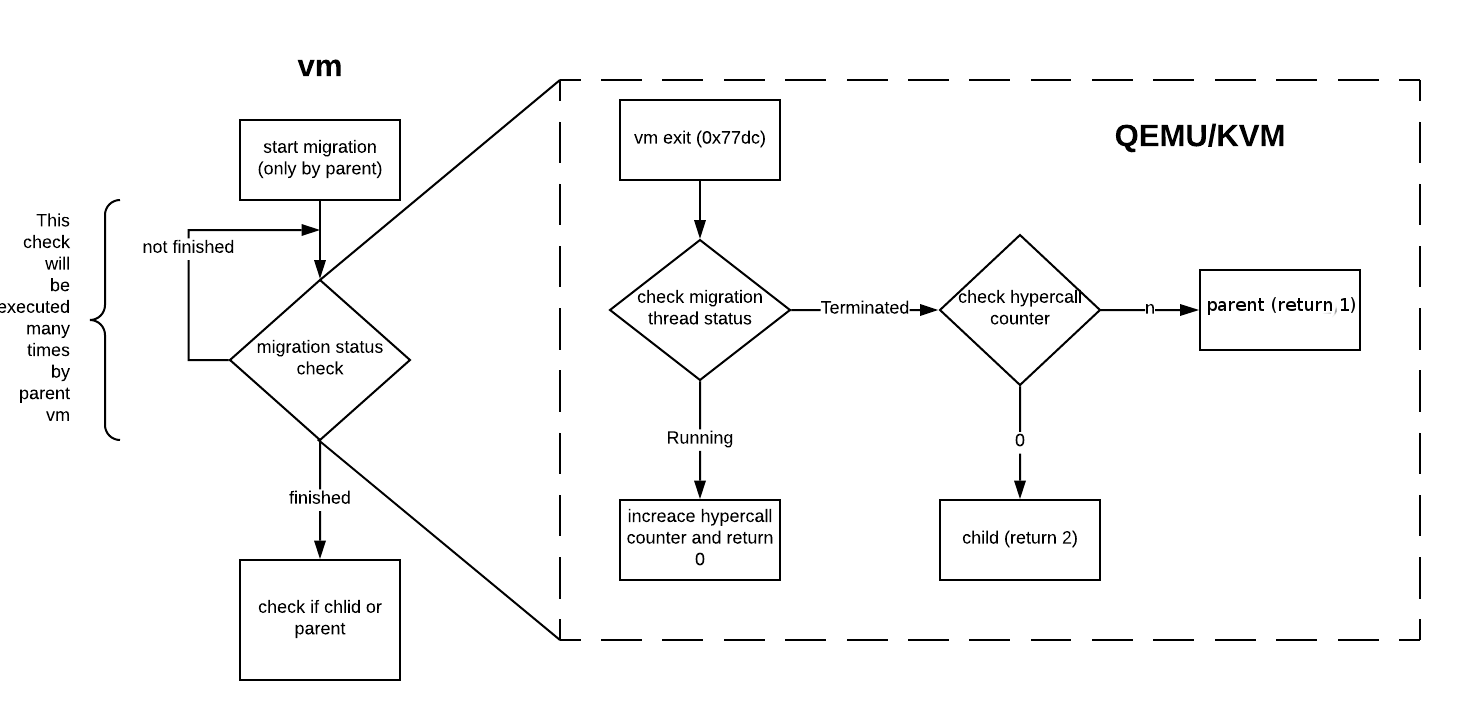
\includegraphics[scale=0.75]{figures/check_migration_status.png}}
\caption{check migration status\label{fig4_9}}
\end{figure}

\subsection{Δημιουργία νέας εικονικής μηχανής}

Έχουμε φτάσει στο σημείο, που έχει τελειώσει η δημιουργία του migration file από
το QEMU και έχει επιστραφεί η τιμή 1 στην εικονική μηχανή αφού πρόκειται για το
γονέα. Το επόμενο στάδιο είναι η δημιουργία του νέου unikernel. Από το γονέα
unikernel γίνεται άλλο ένα hypercall, αλλά σε διαφορετική θύρα την 0x77dc. Το
QEMU λαμβάνοντας το συγκεκριμένο vm exit, ξεκινάει τη διαδικασία για τη
δημιουργία της νέας εικονικής μηχανή. 

Στην περίπτωση του QEMU/KVM κάθε εικονική μηχανή εκτελείται σε ξεχωριστή
διεργασία. Συνεπώς, το πρώτο πράγμα που πρέπει να γίνει είναι η δημιουργία μίας
νέας διεργασίας, η οποία προφανώς γίνεται με τo system call fork. Στη νέα
διεργασία (παιδί) θα εκτελείται το εικονικό μηχάνημα παιδί, ενώ στην
προϋπάρχουσα διεργασία θα συνεχίσει να εκτελείται η εικονική μηχανή γονέας.

Συνεπώς, από τη μεριά της η διεργασία πατέρας, επιστρέφει στην εικονική μηχανή
το process id της νέας διεργασίας και η εικονική μηχανή μπορεί να συνεχίσει την
εκτέλεση της. Από την άλλη η διεργασία παιδί θα πρέπει να ξεκινήσει μία νέα
εικονική μηχανή χρησιμοποιώντας το migration file που δημιουργήθηκε στο
προηγούμενο στάδιο. Η δημιουργία της νέας εικονικής μηχανής γίνεται
χρησιμοποιώντας την κλήση συστήματος execve. Ο μηχανισμός του migration που
διαθέτει το QEMU/KVM απαιτεί, η νέα εικονική μηχανή που θα χρησιμοποιεί το
migration file, να έχει τις ίδιες ακριβώς παραμέτρους με τις οποίες ξεκίνησε η
αρχική εικονική μηχανή. Συνεπώς, οι παράμετροι της execve, είναι ίδιοι με τις
παραμέτρους που ξεκίνησε η αρχική εικονική μηχανή με την προσθήκη tων παρακάτω
επιπλέον επιλογών, που υποδηλώνουν ότι θα χρησιμοποιηθεί το migration file που
δημιουργήθηκε στο προηγούμενο στάδιο.

\begin{lstlisting}[numbers=none]
--incoming  exec: cat /tmp/vm_migration.out 
\end{lstlisting}

Ακόμα, προκειμένου να μην υπάρξει πρόβλημα με την έξοδο του νέου και παλιού
unikernel, ανακτευθύνουμε το stderr και το stdout, της νέας διεργασίας στο
αρχείο "/tmp/my\_server.out". Προφανώς η παραπάνω ενέργεια πρέπει να προηγηθεί
της κλησης execve. 

Το νέο unikernel παιδί θα ξεκινήσει την εκτέλεση του από το προηγούμενο στάδιο,
δηδή θα εκτελέσει ένα hypercall για να ελέγξει αν το migration έχει τελειώσει.
Γίνεται εύκολα κατανοητό, ότι ο μετρητής των hypercalls της διεργασίας παιδί θα
είναι μηδενικός, συνεπώς μόλις το QEMU αναγνωρίσει ότι πρόκειται για το πρώτο
hypercall και ότι δεν εκτελείται το νήμα του migration, θα επιστρεφεί η τιμή 2,
στην εικονική μηχανή. Πλέον υπάρχουν δύο εικονικές μηχανές που κάθε μία γνωρίζει
το ρόλο της (γονέας, παιδί) και μπορούν να συνεχίσουν την κανονική τους λειτουργία.

\subsection{Συγχρονισμός μοιραζόμενης μνήμης}

Στην περίπτωση που χρηιμοποιείται ο μηχανισμός pipe και κατεπέκταση το ivshmem,
παρατηρήσαμε ότι υπάρχει το εξής πρόβλημα. Αν το unikernel παιδί δε γράψει κάτι
στη μοιραζόμενη μνήμη, τότε τα δεοδμένα που γράφονται από το unikernel γονιός
δεν μπορούν να διαβαστούν από το unikernel παιδί. Συνεπώς, απαιτείται κάποιος
συγχρονισμός των δύο unikernels, όσον αφορά τη μοιραζόμενη μνήμη. 

Για την αντιμετόπιση του παραπάνω προβλήματος, αφού το \EN{unikernel} γονιός
εκτελέσει το hypercall για τη δημιουργία της νέας εικονικής μηχανής, αν
χρησιμοποιείται ο μηχανισμός pipe, εκτελεί ακόμα ένα busy wait. Σε αυτό το
σημείο περιμένει να γραφτεί η τιμή 77, σε μία πρκαθορισμένη διευνση της
μοιραζόμενης μνήμης. Μόλις αυτή η τιμή διαβαστεί, τότε η κλήση fork, επιστρέφει
το process id της νέας διεργασίας τυ QEMU και η διαδικασία του fork, έχει
ολοκληρωθεί από τη μεριά του γονέα. 

Αντίστοιχα, το unikernel παιδί, αφού δημιουργηθεί και εκτελέσει το hypercall για
τον έλεγχο του migration θα πρέπει να γράψει την τιμή 77 στη συγκεκριμένη θέση
μνήμης. Προφανώς, η παραπάνω ενέργεια θα εκτελεστεί μόνο στην περίπτωση που
χρησιμοποιείται ο μηχανσιμός pipe. Από εκεί και πέρα και το unikernel παιδί,
έχει ολοκληρώσει και αυτό τη διαδικασία του fork και επιστρέφοντας την τιμή 0,
δίνει τον έλεγχο στην εφαρμογή να συνεχίσει την εκτέλεση της.

\subsection{Σύνοψη}

Στην παρακάτω εικόνα ~\ref{fig4_11} φαίνονται με χρονολγοική σειρά τα στάδια
την υλοποίηση του μηχανσιμού fork. Προφανώς τα βήματα μετά το fork, μπορεί να
μην έχουν ακριβώς αυτή τη σειρά, καθώς αυτή εξαρτάται από τη χρονοδρομολόγηση
των εικονικών μηχανών και του QEMU. Συνοψίζοντας τα βήματα έχουν ως εξής:
\begin{enumerate}
	\item Το unikernel γονέας, κάνει hypercall στο QEMU για την εκκίνηση της
		δημιουργίας του migration file 
	\item Το unikernel γονέας, περιμένει την ολοκλήσρωση του migration. Όταν
		ολοκληρωθεί, θα του επιστραφεί η τιμή 1.
	\item Το unikernel γονέας, κάνει νέο hypercall στο QEMU για τη
		δημιουργία νέας εικονικής μηχανής. 
	\item Το qemu κάνει fork. Στο γονέα επιστρέφει το process id της νέας
		διεργασίας qemu. Η διεργασία παιδί εκτελέι execve για την
		εκκίνηση της νέας εικονικής μηχανής χρησιμοποιώντας το migration
		file που δημιουργήθηκε. 
	\item Το unikernel γονέας, περιμένει να συγχρονίσει την μοιραζόμενη
		μνήμη, αν υπάρχει.
	\item Το unikernel παιδί, ελέγχει αν έχει τελειώσει το migration και του
		επιστρέφεται η τιμή 2.
	\item Το unikernel παιδί συγχρονίζει την κοινή μνήμη.
\end{enumerate}

\begin{figure}[htp]
\centerline{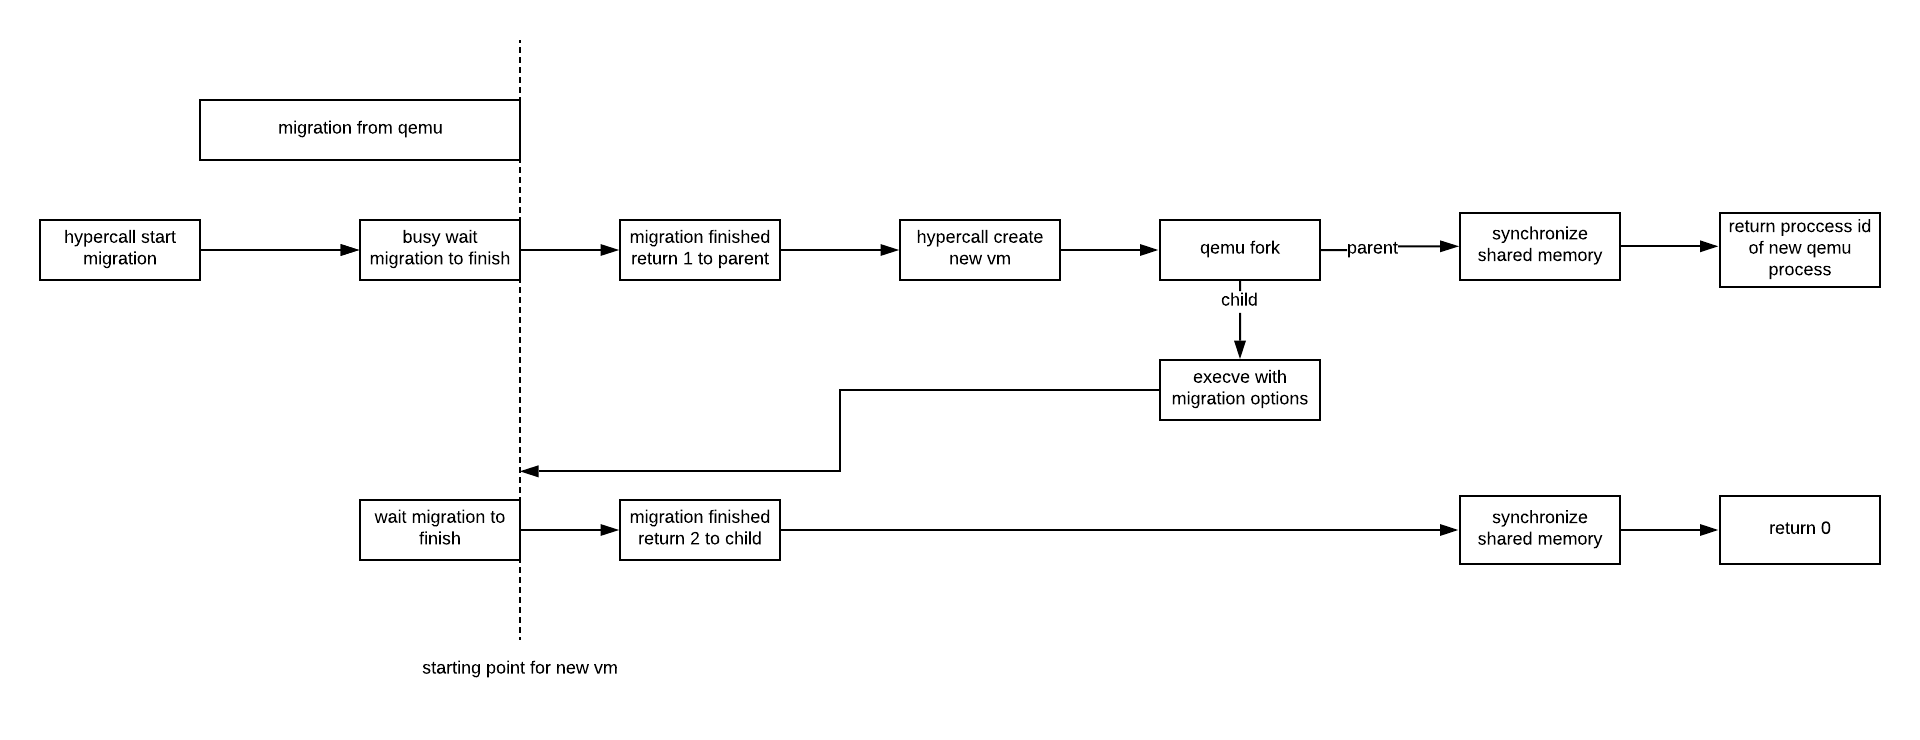
\includegraphics[scale=0.6]{figures/fork_timeline.png}}
\caption{fork steps\label{fig4_11}}
\end{figure}

Προκειμένου να αξιολογήσουμε τη συγκεκριμένη υλοποίηση, θα συγκρίνουμε τους
χρόνους που χρειάζεται η ίδια εφαρμογή για να κάνει fork σε λειτουργικό συτημα
linux και στο Rumprun unikernel. Και στις δύο περιπτώσεις, τα λειτουργικά
συστήματα εκτελούνται πάνω στην ίδια έκδοση qemu. Το πρόγραμμα που
χρησιμοποιήθηκε και στις δύο περιπτώσεις φαίνεται στο τέλος του κεφαλαίου και
δεν κάνει χρήση του μηχνασιμού pipe. Οι μετρήσεις έγιναν σε υπολογιστή με
λειτουργικό σύστημα Linux 3.16.0-6-amd64 \#1 SMP Debian 3.16.56-1+deb8u1, με
επεξεργαστή Intel(R) Core(TM)2 Duo CPU P8400. Στην περίπτωση του linux η
εφαρμογή για να κάνει fork, χρειάζεται 0.000138s,  ενώ στην περίπτωση του
rumprun, χρειάζεται 0.137423s. 

Παρατηρούμε μία πολύ μεγάλη διαφορά μεταξύ τν δύο περιπτώσεων. Η διαφορά αυτή
δικαιολογείται από το γεγονός ότ στη μία περίπτωση, δημιουργείται μία νέα
διεργασία, ενώ στην άλλη μία ολόκληρη εικονική μηχανή. Μάλιστα στην περίπτωση
του RUmprun, πρέπει να δημιουργηθεί, το migration file και ύστερα να
δημιουργηθεί μία νέα QEMU διεργασία η οποία θα εκκινήσει τη νέα εικονική μηχανή
με βάση το migration file. Προκειμένου, να δούμε γιατί είναι τόσο αργό το fork,
στην περίπτωση του QEMU, μετρήσαμε κάθε ένα από τα βήματα που εκτελούνται από 
το μηχανσιμό. 
Στο παρακάτω σχήμα ~\ref{fig4_12} φαίνεται, το ποσοστό του χρόνου που
λαμβάνει κάθε βήμα.

\begin{figure}[htp]
\centerline{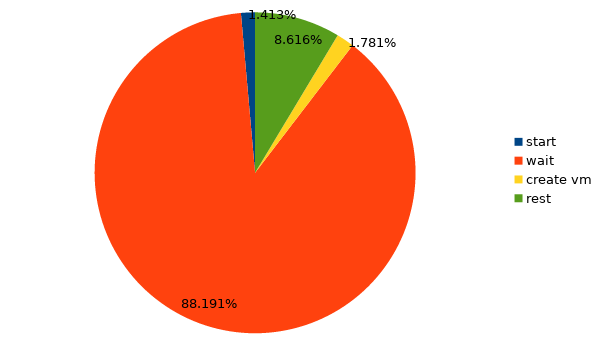
\includegraphics[scale=0.8]{figures/fork_pie.png}}
\caption{Time for each step in fork mechanism\label{fig4_12}}
\end{figure}

\newpage
\begin{lstlisting}
#include <sys/stat.h>
#include <fcntl.h>
#include <unistd.h>
#include <stdio.h>
#include <stdlib.h>

#include <sys/time.h>
#define USEC            1000000

int main()
{
        int fd[2], n;
        struct timeval t1, t2;
        gettimeofday(&t1, 0);
        n = fork();
        if (n == 0) {
                /* child */
                gettimeofday(&t2, 0);
                printf("child: fork took: %lfs\n", (double)((t2.tv_sec - t1.tv_sec) * USEC + t2.tv_usec - t1.tv_usec) / USEC);
        } else if (n < 0) {
                perror("fork");
                exit(1);
        } else {
                gettimeofday(&t2, 0);
                printf("parent: fork took: %lfs\n", (double)((t2.tv_sec - t1.tv_sec) * USEC + t2.tv_usec - t1.tv_usec) / USEC);
        }
        return 0;
}

\end{lstlisting}
